\documentclass[10pt,letterpaper]{article}
\usepackage{cogsci}
\usepackage{pslatex}
\usepackage[nodoi]{apacite}
\usepackage{amsmath, amssymb}
\usepackage{graphicx}
\usepackage{caption}
\usepackage{subcaption}
\captionsetup[subfigure]{labelformat=brace}
\usepackage{tabulary}
\usepackage{natbib}
\usepackage{multirow}
\usepackage{rotating}
\usepackage{times}
\usepackage{csquotes}
\usepackage{calc}
\usepackage[bottom]{footmisc}
\usepackage[font=footnotesize,skip=6pt]{caption} %smaller caption font
\def\bibfont{\footnotesize}



\usepackage{color}
\definecolor{Green}{RGB}{10,200,100}
\newcommand{\ndg}[1]{\textcolor{Green}{[ndg: #1]}}  
\newcommand{\as}[1]{\textcolor{blue}{[ast: #1]}}
\newcommand{\todo}[1]{\textcolor{red}{[TODO: #1]}}
\newcommand{\demi}[1]{\textcolor{magenta}{[demi: #1]}} 

\makeatletter
\def\hlinewd#1{%
\noalign{\ifnum0=`}\fi\hrule \@height #1 %
\futurelet\reserved@a\@xhline}
\makeatother

\title{Gauging Compositionality in Sentence Embeddings}
 
\author{\textbf{Ishita Dasgupta$^1,$  Demi Guo$^4,$ Andreas Stuhlm\"uller$^2,$ Samuel J. Gershman$^3$ \& Noah D. Goodman$^2$}\medskip\\ 
$^1$Department of Physics and Center for Brain Science, Harvard University\\
$^2$Department of Psychology, Stanford University\\
$^3$Department of Psychology and Center for Brain Science, Harvard University\\
$^4$Department of Computer Science, Harvard University
}


\begin{document}

\maketitle


\begin{abstract}
Word embeddings trained on large corpora are frequently used as features for NLP systems. Recent research has attempted to generate such vector space embeddings for larger pieces of text, such as sentences and paragraphs. The understanding of language and the combinatorially large number of possible sentences hinges on the ability to understand the systematic compositionality of how words combine. While these vector representations of sentences outperform bag-of-words models on several tasks, it is unclear how much compositionality they truly capture. We present a dataset for a natural language inference task that cannot be solved using only lexical/word level knowledge and instead requires varying degrees of compositionality. We use sentence embeddings from InferSent \citep{Conneau:2017uf}, the state of the art in sentence level transfer tasks, and find that performance on our tasks is poor, indicating that the representations induced by this model capture little compositionality. We analyze what limited compositionality is in fact learned by InferSent (affording it higher performance on NLI than bag-of-words models) and find that it is largely driven by some simple heuristics at the word level that are ecologically valid in the SNLI dataset. This highlights the potential difficulties in training such general purpose function approximators such as RNNs for a task as complex and specific as understaning language, and the importance of having structured datasets in better understanding the performance of these systems (as well as in improving their performance).
\textbf{Keywords:} 
Sentence embeddings; compositionality; test data sets
\end{abstract}


\section{Introduction and Motivation}
In the world of deep learning, statistical structure is extracted by training on very large datasets. Several of these models are in theory Turing complete, leaving the discovery of the right parameters mostly to the training data and partially also to the training protocols. The training datasets are assumed to be samples from the natural distribution. While it remains an interesting question as to whether these training data sets truly are sampling the true distribution we want to approximate, another question is of how many random samples from the true distribution are enough to sufficiently constrain the space of models (in the huge space of possibilities the thousands of parameters in a neural network model allow) that explain the training data. Heuristics literature shows that simple strategies often satisfactorily explain the bulk of the variance amongst the most likely scenarios.

\textbf{discussion on heuristics literature}

Perhaps a better strategy for generating training data is to sample the cases that are most informative about the validity of competing models, especially to help rule out simple heuristics. This necessitates the disproportionate representation of `edge cases' that do not have high probability of occurrence in the wild i.e. when sampling from the natural distribution. The creation of such "teaching" data sets better constrain the set of the possible models, instead of blindly sampling from the distribution posited by the true model.

\textbf{discussion on ``teaching data sets"}

It is not a new proposal that one should focus on the boundaries when trying to learn structures, this has parallels to research on adversarial training. However, in the realms of very structured compositional domains like language, perhaps it is unrealistic to generate good adversarial examples that are valid. Enter the field of cognitive psychology and psycholinguistics where people have been coming up with good edge cases to test human understanding of these domains for decades. 

\textbf{discussion on what cogsci can offer / why adversarial training as it stands isn't there yet}

The disproportionate sampling of tails of the true distribution, and the contrived cases that live there, is unlikely to occur in a natural environment. Perhaps kids are given some extra exposure to common pitfalls etc and what to avoid during schooling and other pedagogy, but it is disheartening to believe that structures cannot be learned from passive observation of natural statistics. However, generative learners are less sensitive to variations in the distributions of observed data and make better use of implicit negative evidence. So perhaps this kind of hand-holding is not necessary for more generative models.


\section{Sentence Encoding}

Understanding language requires the understanding not just of the words, but of their relation and ordering in a sentence. Models of word semantics where words are embedded in a vector space have been successful in capturing the meanings of words. However, due to the combinatorial productivity of language, the number of possible sentences far exceeds the size of the vocabulary, and generating similar vector embeddings for sentences has proved challenging. Recent literature reports several supervised as well as unsupervised approaches to learning sentence representations using Recurrent Neural Networks that account for word ordering \citep{Kiros:2015uq, Hill:2016uu, Conneau:2017uf}. 
% Consider commenting on neural Turing machine type thing - i.e. nn with memory?
These are intended to capture their semantic content, and perform reasonably well on transfer tasks---i.e. other semantic tasks which the embeddings were not specifically trained on. Particularly, the performance of these sentence models on these tasks supersedes the performance of bag-of-words models that patently lack any relational information about the words, i.e. lack any compositionality. However, it is unclear exactly what kind of compositional information is gained in these sentence models, above lexical meaning. We try to address this question by designing a dataset that relies on increasing degrees of compositional information, and is intractable for systems that capture only lexical information. Further, we try to characterize the compositional information in these sentence embeddings by understanding the cases where the sentence models succeed but the BOW models fail. Based on our observations, we hypothesize that the reason InferSent or modern neural network models fail to learn the compositionality of sentences is that they heavily rely on the data distribution, and overgeneralize patterns in training data. Given the exponentially large number of possible sentences, most subsets of sentences unless meticulously designed, can be justified by heuristics simpler than the true generative process of language. We analyze these heuristics and find their ecological validity in the SNLI dataset.  Finally, we retrain a model on a dataset combining our ScrambleTest set and original SNLI train set to see if structured datasets like ours can be learned by the InferSent architecture.

\section{NLI classifier}
The sentence embeddings we use are from InferSent \citep{Conneau:2017uf}. We choose to use these sentence embeddings as they hold the current state of the art for transfer in semantic tasks, and we expect that strong performance in transfer tasks indicates a good representation for the semantics of a sentence. These embeddings were trained end-to-end using the architecture in Figure \ref{fig:arch} on the SNLI training set \citep{snli:emnlp2015}. The training tasks is to classify pairs of sentences into `entailment', `contradiction', or `neutral'. The embeddings were shown to perform well on other tasks (such as sentiment analysis, semantic textual similarity and other natural language inference datasets) by re-using the embedding layers and training only the classifier for the specific task at hand. In the following, we use the pre-trained embeddings made available by the authors, featurized as suggested. We trained a classifier on the SNLI training set independently (using logistic regression as well as multilayer perceptron with a single hidden layer), with regularization optimized on the SNLI validation set. The bag of words (BOW) baseline model averages the GloVe embeddings for all the words in the sentence to form a sentence embedding. The BOW-LR and BOW-MLP achieve $50.24\%$ and $53.99\%$ accuracy respectively and the InferSent embeddings (LR and MLP) achieve $83.61\%$ and $83.45\%$ accuracy, on the SNLI test set (comparable to the performance in the end-to-end trained classifier as reported in \cite{Conneau:2017uf}). Details of The logistic regressions are in Figures \ref{fig:SNLIBOWhist} and \ref{fig:SNLIIShist}, MLP results look qualitatively similar.

\begin{figure}[ht!]
\centering
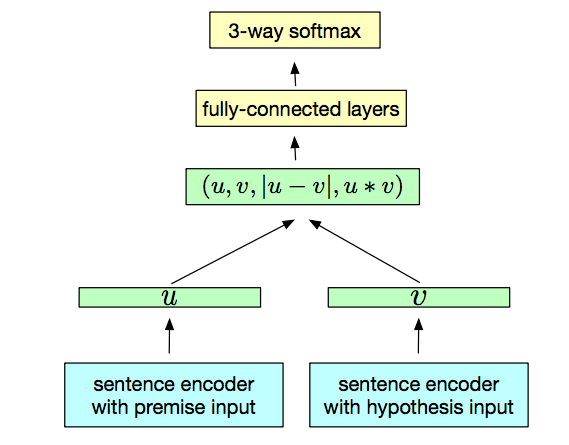
\includegraphics[width=0.4\textwidth]{InferSent_arch.png}
\caption{InferSent architecture. Source \citet{Conneau:2017uf}}
\label{fig:arch}
\end{figure}

\begin{figure}[ht!]
\centering
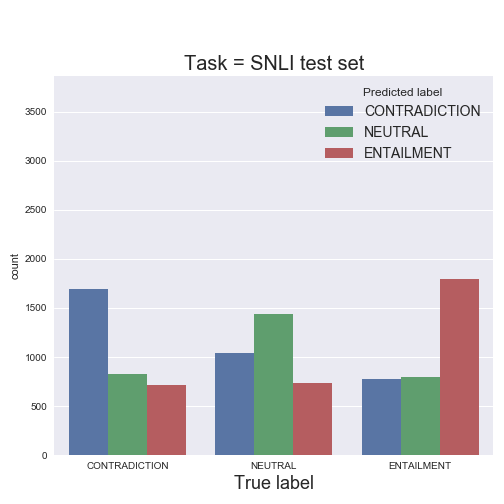
\includegraphics[width=0.35\textwidth]{SNLIBOWLogRegHistAll.png}
\caption{SNLI test Data: Logistic regression on BOW embeddings}
\label{fig:SNLIBOWhist}
\end{figure}


\begin{figure}[ht!]
\centering
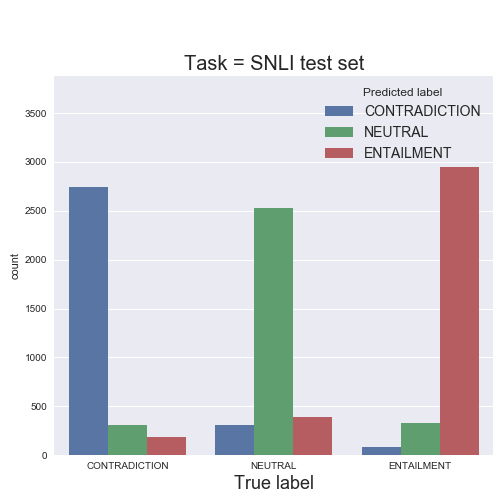
\includegraphics[width=0.35\textwidth]{SNLIInferSentLogRegHistAll.png}
\caption{SNLI test Data: Logistic regression on InferSent embeddings}
\label{fig:SNLIIShist}
\end{figure}

\bgroup
\def\arraystretch{1.5}
\begin{center}
 \begin{tabular}{||p{30mm} c||} 
 \hline
 Type & Number of sentence pairs \\ [0.5ex] 
 \hline\hline
 Adjective-Referent binding & 9600  \\
 \hline
 Adjective-Referent binding (who is) & 9600  \\
 \hline
 Comparisons (more/less)  & 4800 \\
 \hline
 Comparisons (not)  & 9600 \\
 \hline
 Comparisons (same)  & 9600 \\
 \hline
 Negating Condition & 144 \\[1ex] 
 \hline
 Temporal ordering & 1600 \\
 \hline
 Subject-Verb binding & 2400 \\ 
 \hline
 Verb Symmetry (contradiction) & 200 \\ 
 \hline
 Verb Symmetry (neutral) & 200 \\ 
 \hline
 
\end{tabular}
\end{center}


\section{Test data set}
Our goal is to design sets of pairs of sentences such that the relation within a pair (entailment, neutral or contradiction) can be changed without changing the words involved, simply by changing the word ordering within each sentence.

There are different levels of difficulty in the kinds of tasks we consider. The datasets are made up of two sets of sentence pairs, with two different relationships (of entailment, contradiction and neutral), such that the words in each sentence of the pair are the same across the set, but are reordered. Each data-set consists of such sets of sentence pairs, so that there are equal numbers of sentence pairs with two different relationships (among entailment, neutral and contrdiction).\\
Therefore, the maximum possible performance of a bag of words model is $50\%$, since it cannot distinguish the two pairs in the set, and cannot classify them differently. This provides a hard baseline for the performance that is possible without compositional understanding. Any performance above the BOW model is often seen as proof of compositionality. However, this is an unfair comparison – the bag of words model baseline as implemented for comparsons receives only averaged word vectors for the sentence and therefore theoretically also loses some of the lexical information.  We can gauge the compositionality that InferSent learns by seeing how differently it classifies these scrambled sets, and measuring its performance above $50\%$. Further, we make two copies of each dataset, one with exclusively short noun phrases (eg. `the boy'), or long noun phrases (eg. `the boy holding an umbrella') as a control to see how length affects performance.

\subsection{Verb Symmetry}

Some verbs are symmetric and some are not in terms of the subject and the object. We can form pairs of sentences by exchanging the subject and the object that have entailment, contradiction, or neutral relationships. We have 2 subcategories of these kinds of examples.

\subsubsection{Contradiction type}
Where the word reordering changes the relationship from entailment to contradiction.\\
{ \tt A: The woman overtakes the man \\ B: The woman overtakes the man \\ ENTAILMENT \\}{\tt A: The woman overtakes the man \\ B: The man overtakes the woman \\ CONTRADICTION }

\subsubsection{Neutral type}
Where the word reordering changes the relationship from entailment to neutral.\\
{ \tt A: The woman watches the man \\ B: The woman watches the man \\ ENTAILMENT \\}{\tt A: The woman watches the man \\ B: The man watches the woman \\ NEUTRAL }

\subsection{Comparisons}

When comparing two entities, the order of the entities matters in the sentence. We have 3 subcategories of comparisons.
\subsubsection{More-Less type}
Where the A-B pairs in each pair of sentence differ by whether they contain the word `more' or the word `less'. \\
{\tt A: The woman is more cheerful than the man \\ B: The woman is less cheerful than the man\\ CONTRADICTION \\}{\tt A: The woman is more cheerful than the man \\ B: The man is less cheerful than the woman \\ ENTAILMENT} 

\subsubsection{Not type}
Where the A-B pairs in each pair of sentence differ by whether they contain the word `not'. \\
{\tt A: The woman is more cheerful than the man \\ B: The woman is not more cheerful than the man\\ CONTRADICTION \\}{\tt A: The woman is more cheerful than the man \\ B: The man is not more cheerful than the woman \\ ENTAILMENT} 


\subsubsection{Same type}
Where the A-B pairs in each pair of sentence differ only in the order of the words. \\
{\tt A: The woman is more cheerful than the man \\ B: The woman is more cheerful than the man\\ ENTAILMENT \\}{\tt A: The woman is more cheerful than the man \\ B: The man is more cheerful than the woman \\ CONTRADICTION } 

\subsection{Temporal ordering}

Indication of the relative temporal ordering of events is also sensitive to the ordering of the same words in the sentence.\\
{\tt  A: The woman stood up after the man stood up \\ B: The woman stood up after the man stood up \\ ENTAILMENT \\}{\tt A: The woman stood up after the man stood up \\ B: The man stood up after the woman stood up \\ CONTRADICTION}

\subsection{Adjective-Referent binding}
To keep track of which noun in the sentence an adjective is referring to, the order of the words is critical.\\
{\tt A: The tall woman met the short man \\ B: The woman met the short man \\ ENTAILMENT \\}{\tt A: The tall woman met the short man \\ B: The short woman met the man \\ CONTRADICTION}\\

\subsubsection{With who-is} 
We include a variant in which the adjective is bound to the referent with "who is". \\
{\tt A: The woman who is tall met the man who is short \\ B: The woman met the man who is short \\ ENTAILMENT \\}{\tt A: The woman who is tall met the man who is short \\ B: The woman who is short met the man\\ CONTRADICTION}

\subsection{Subject-Verb binding}
In phrases where two subjects do different things, it is required that the relative relation between the verb and noun phrases be retained.\\
{\tt A: The woman stands up, however the man sits down \\ B: The woman stands up. \\ ENTAILMENT \\}{\tt A: The man stands up, however the woman sits down \\ B: The woman stands up. \\ CONTRADICTION}

\subsection{Negating a condition}
There is unequal effect of negating the condition for a phenomena or the phenomena itself. \\
{\tt A: If there is a lot of snow, it is very cold \\ B: If there is a lot of snow, it is not very cold \\ CONTRADICTION \\}{\tt A: If there is a lot of snow, it is very cold \\ B: If there is not a lot of snow, it is very cold \\ NEUTRAL}

% \setlength{\arrayrulewidth}{.2em}
% \hlinewd{2pt}
\bgroup
\def\arraystretch{1.5}
\begin{center}
\begin{table}[ht!]
  \begin{tabular}{||l | l | l | l | l | l ||}
    \hline
    \multicolumn{2}{||c|}{Type} &
      \multicolumn{2}{c|}{BOW} &
        \multicolumn{2}{c||}{InferSent}\\
     
    \multicolumn{2}{||c|}{}&LogReg & MLP & LogReg & MLP \\
     \hline
     
     
    \multirow{2}{*}{Adj-ref} &long&39.2&50&51.91&\textbf{51.39} \\
    \cline{2-6}
     &short& 49.71& 50& 53.25&\textbf{54.38} \\
     \hline
    
    \multirow{2}{*}{\parbox{1.3cm}{Adj-Ref (who is)}}  &long& 37.04& 49.83& 65.81& \textbf{64.67} \\
    \cline{2-6}
     &short&49.54& 50& 72.06& \textbf{72.34} \\
     \hline
    
    
    \multirow{2}{*}{\parbox{1.4cm}{Comp (more/less)}} &long&0.08&7.38&43.10&\textbf{50.46} \\
    \cline{2-6}
     &short&4.5&18.79&42.73&49.69 \\
     \hline
    
    \multirow{2}{*}{\parbox{1.3cm}{Comp (not)}} &long&3.15&45.38&42.54&39.38 \\
    \cline{2-6}
     &short&37.31&49.98&31.94&34.96 \\
     \hline
    
    \multirow{2}{*}{\parbox{1.3cm}{Comp (same)}} &long&12.44&50&50&\textbf{50.79} \\
    \cline{2-6}
     &short&47.58&50&66.83&\textbf{79.81} \\
     \hline
     
     \multicolumn{2}{||c|}{Neg-Cond} &1.39&0&14.58&34.72 \\
    \hline
    
    \multirow{2}{*}{\parbox{1.3cm}{Subj--Verb}} &long&36.08&46.58&\textbf{53.17}&50.75 \\
    \cline{2-6}3
     &short&47.25&50&53.79&\textbf{56.17} \\
     \hline

	\multirow{2}{*}{\parbox{1.3cm}{TempOrd}} &long&17.5&50&50&50 \\
    \cline{2-6}
     &short&35.5&50&50&50 \\
     \hline


	\multirow{2}{*}{\parbox{1.3cm}{VerbSym (contr)}} &long&20&50&51&50.5 \\
    \cline{2-6}
     &short&45&50&63&\textbf{63.5}  \\
     \hline
    
    \multirow{2}{*}{\parbox{1.3cm}{VerbSym (neut)}} &long&50&50&50&50\\
    \cline{2-6}
     &short&50&50&50&50\\
     \hline
    
    
     \hline
  \end{tabular}
 
\end{table}
\end{center}



\section{Experiments}
We first do the analysis based on the percentage of correct classifications obtained by each of the 4 classifiers we have -- MLP (with one hidden layer) trained on InferSent embeddings or trained on averaged GloVe embeddings, i.e. the Bag-of-Words baseline, as well as a logistic regression trained on each of these embeddings.
\begin{figure}[t!]
\centering
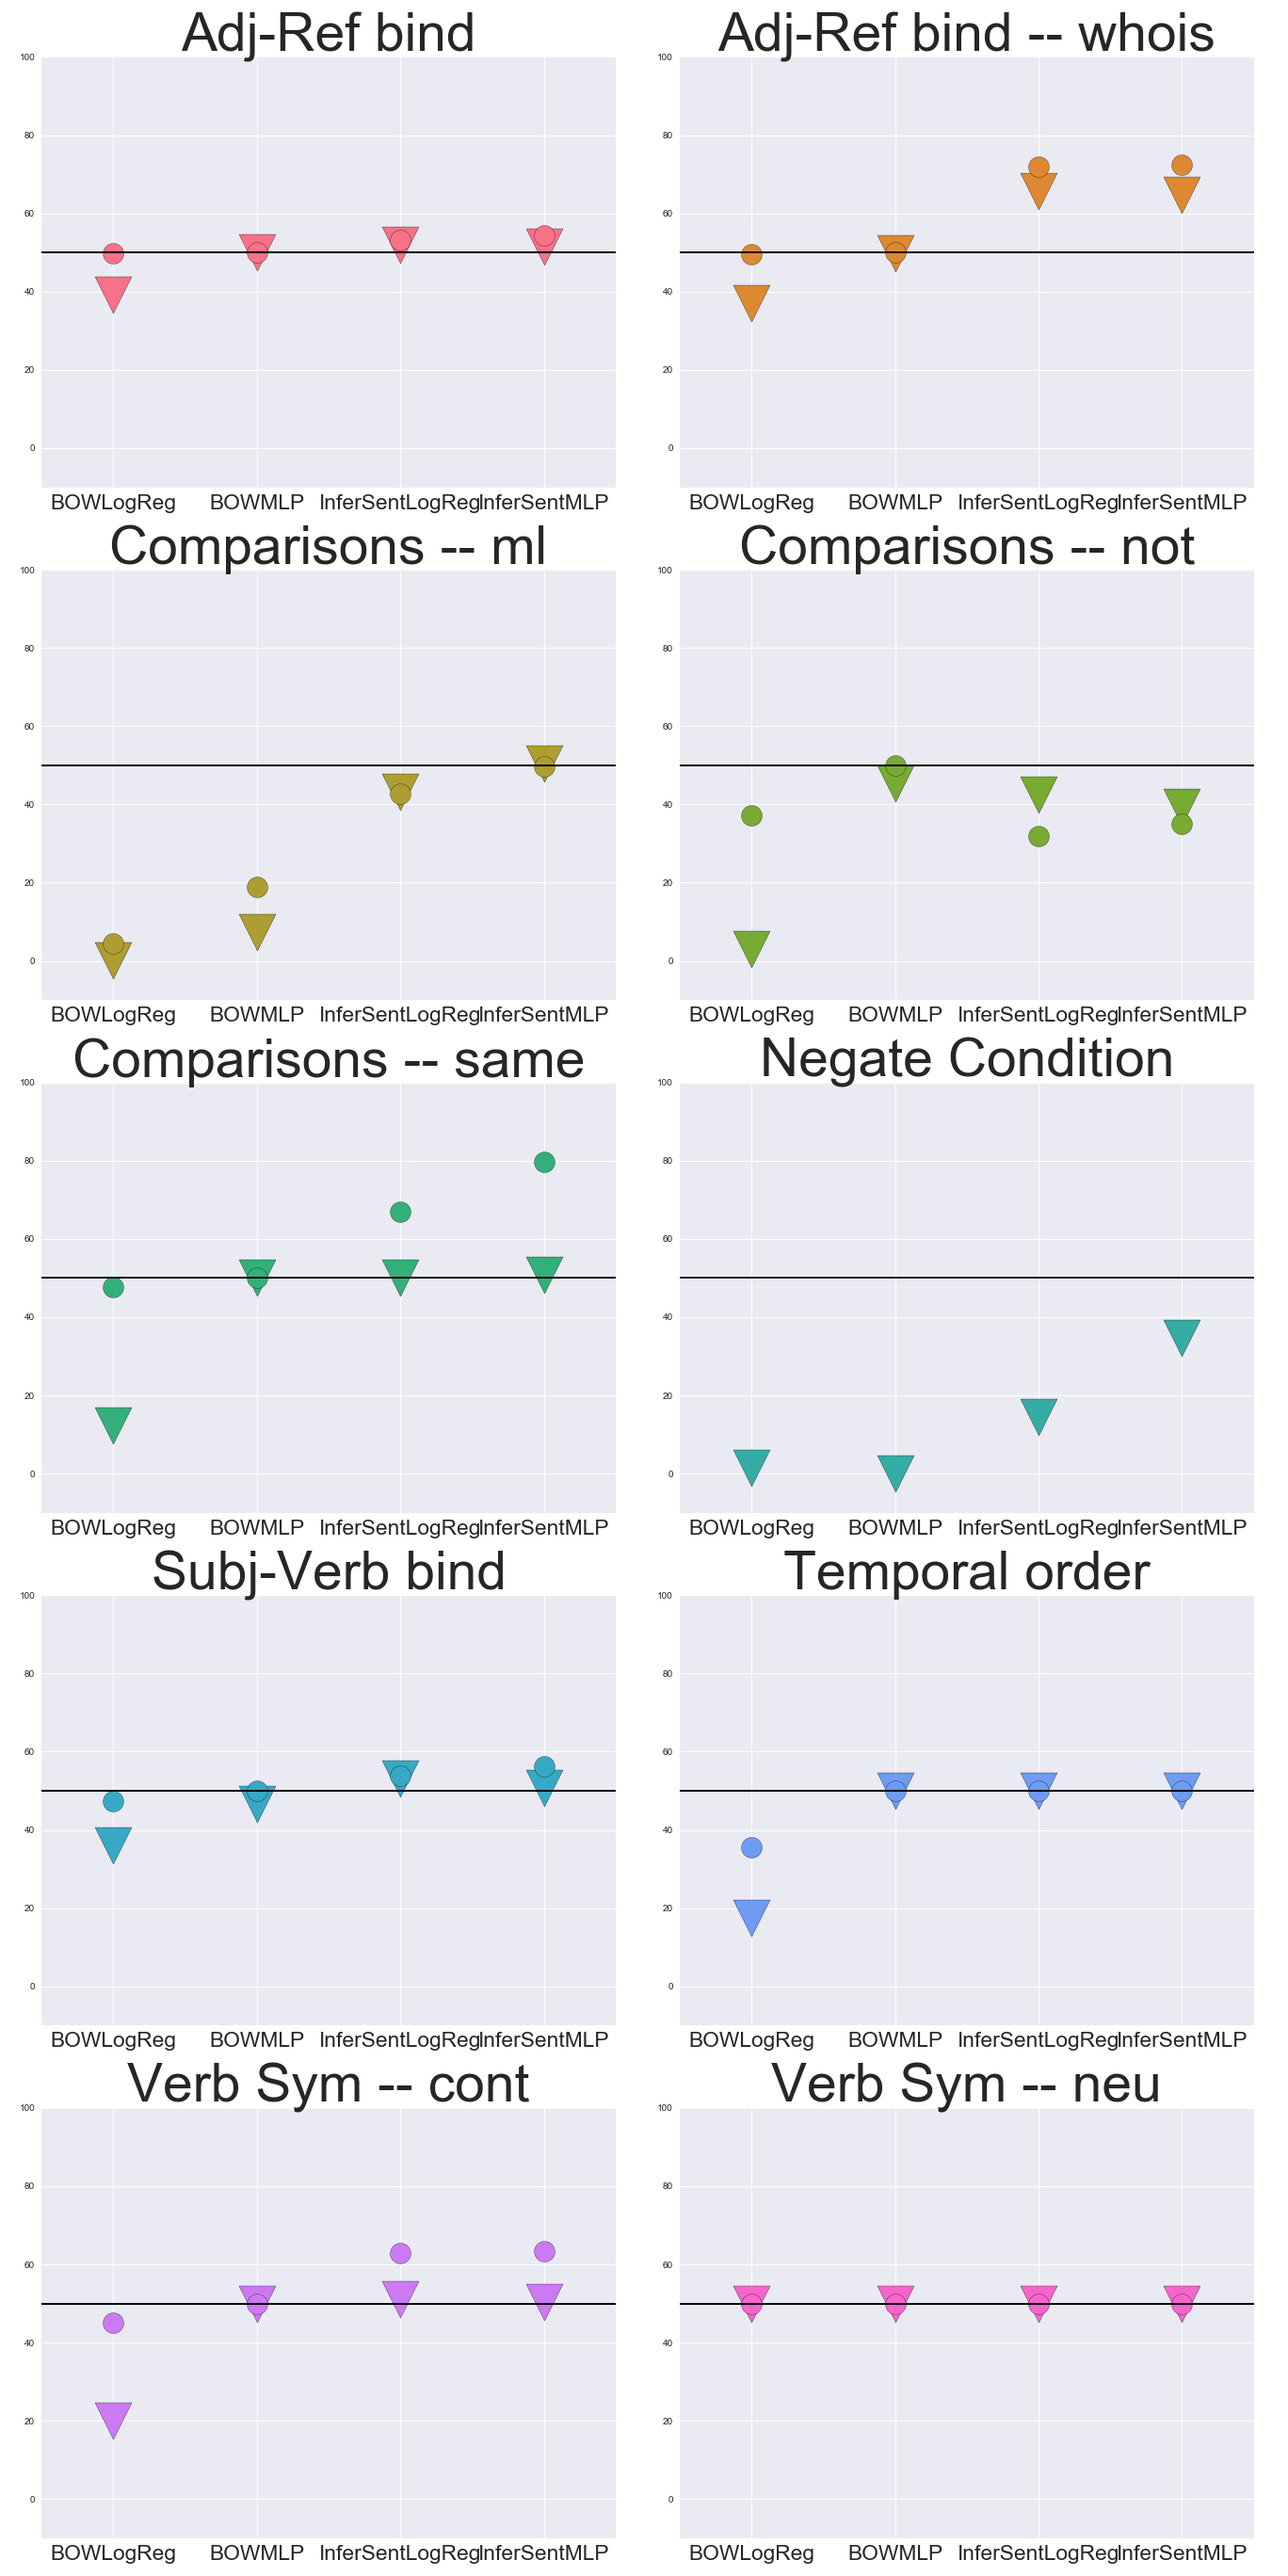
\includegraphics[width=0.45\textwidth]{AllTasks.png}
\caption{Performance on all tasks in ScrambleTest. Triangles represent `long' noun phrases, circles represent `short' noun phrases}
\label{fig:AllTasks}
\end{figure}

We see that, as expected, BOW never exceeds $50\%$ precision. In fact, BOW thinks almost all of the pairs are entailments. The MLP performs better than the LogReg in general, although their performance on the SNLI test set was close to identical. 


\begin{figure}[t!]
\centering
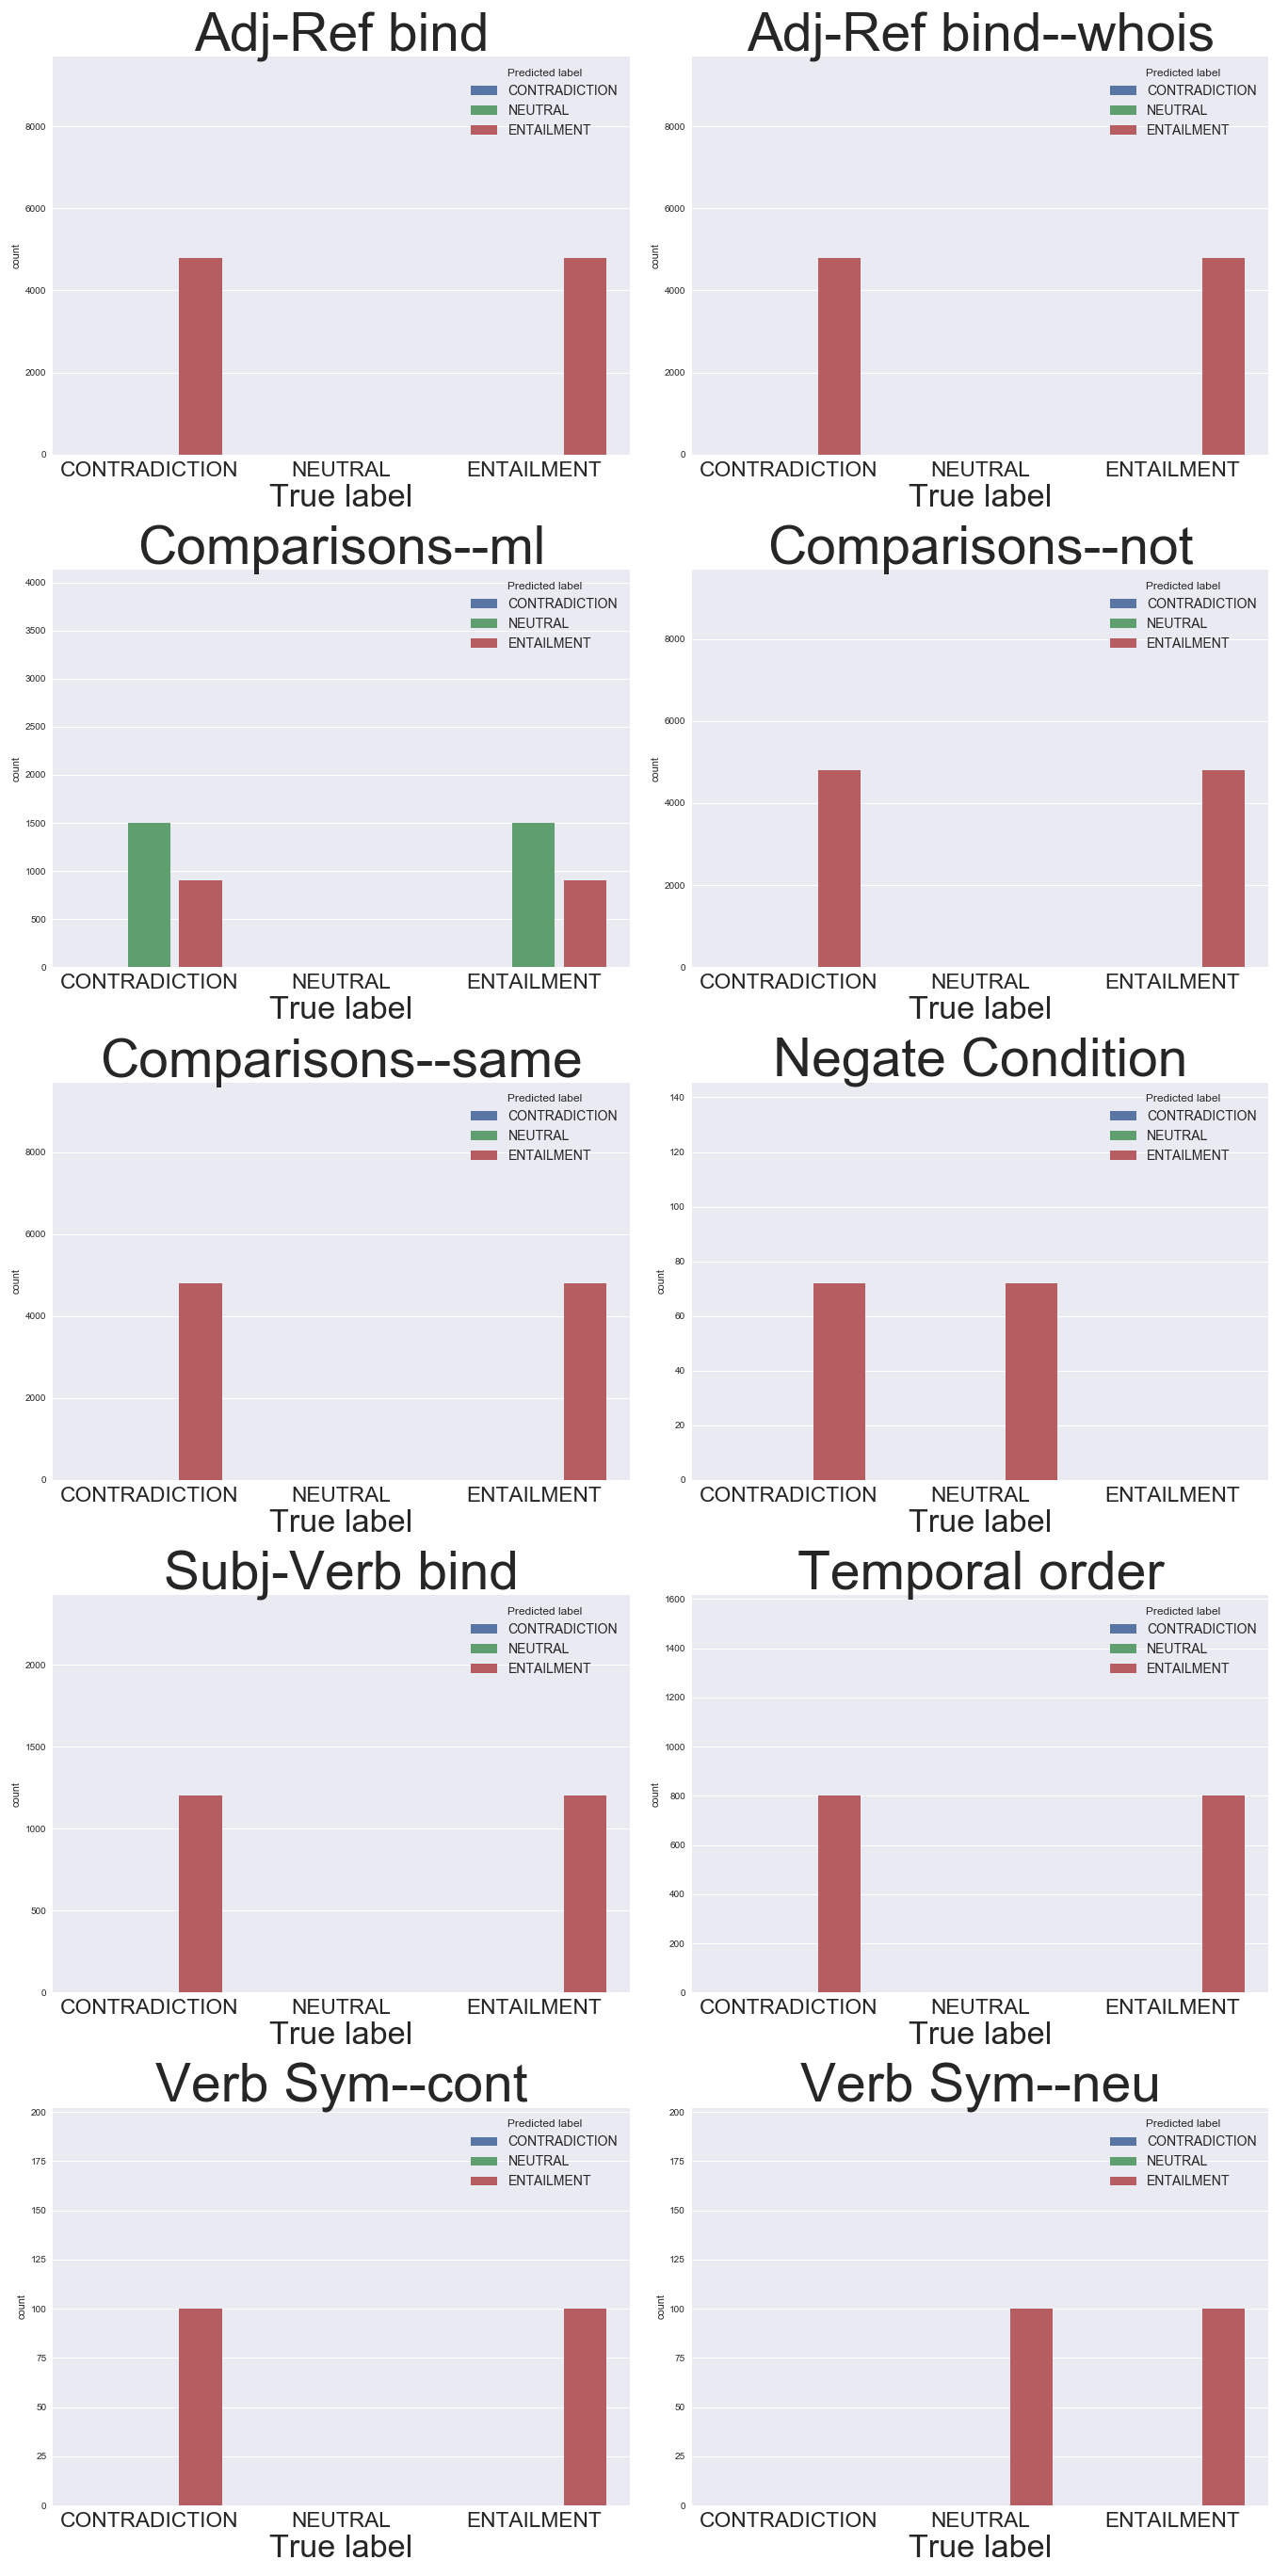
\includegraphics[width=0.45\textwidth]{AllHistsBOWMLPshorts.png}
\caption{The classifications made by the MLP on the BOW vectors. The symmetries across the classifications are clear.}
\label{fig:BOWhistMLPshorts}
\end{figure}

\section{Classification Analysis}

In order to better understand InferSent's performance, we look at the specific classifications it makes. We just consider the MLP results on short noun phrases. Resulst for long noun phrase, and both results for logistic regression results are in the appendix. We see that for BOW, the classifications made are exactly symmetric across the two true categories in each task (Figure \ref{fig:BOWhistMLPshorts}) by design, since members of each category are just scrambled versions of each other and BOW cannot distinguish them. A sign of using more than word-level information is the asymmetry between the classifications of the two categories.

We divide the performance of InferSent into three categories – `high asymmetry, high scores' where more than word level information is used to make the right inferences, `high asymmetry (Figure \ref{fig:IShistMLP-PP}), low success' where more than word level information is used, but not to make the right inferences (Figure \ref{fig:IShistMLP-NP}), `low asymmetry, low success' where InferSent fails to use more than word level information (Figure \ref{fig:IShistMLP-NN}). Here we designate `high' perfromance very loosely to anywhere with more than $50\%$ scores. We choose this set of distinctions because not using more than word level information will ensure bad performance on these tasks, but use of more than word level information doesn't guarantee good performance. This is because each task consists of members of two classes, but there are 3 classes into which the classifier can place each pair. Classification into the third class will always result in low performance, even if the classification differentially uses more than word level information (i.e. if there is high asymmetry).

\begin{figure}[ht!]
\centering
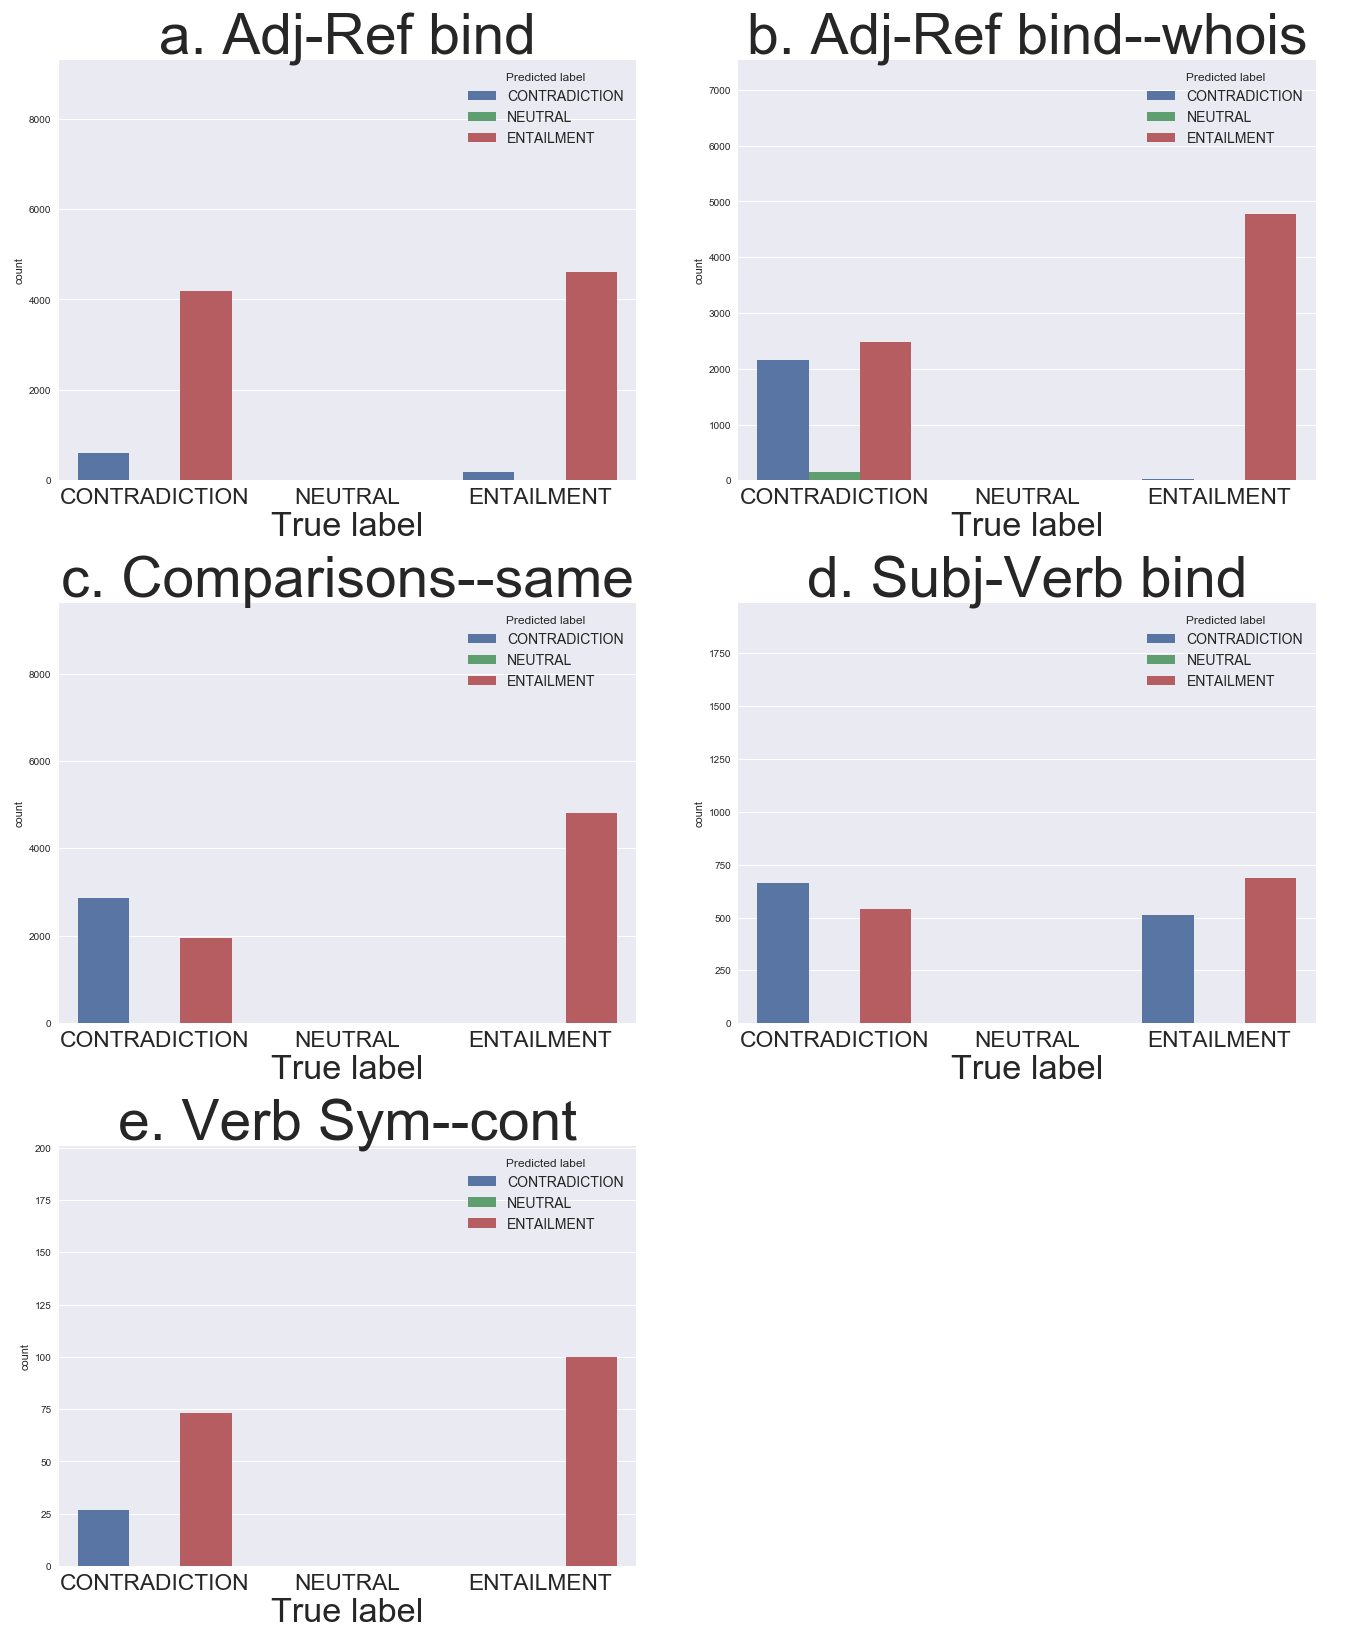
\includegraphics[width=0.45\textwidth]{PPShortHistsInferSentMLP.png}
\caption{Classifications by the MLP on the InferSent vectors with short noun phrases, tasks with `high asymmetry, high scores'.}
\label{fig:IShistMLP-PP}
\end{figure}


\begin{figure}[ht!]
\centering
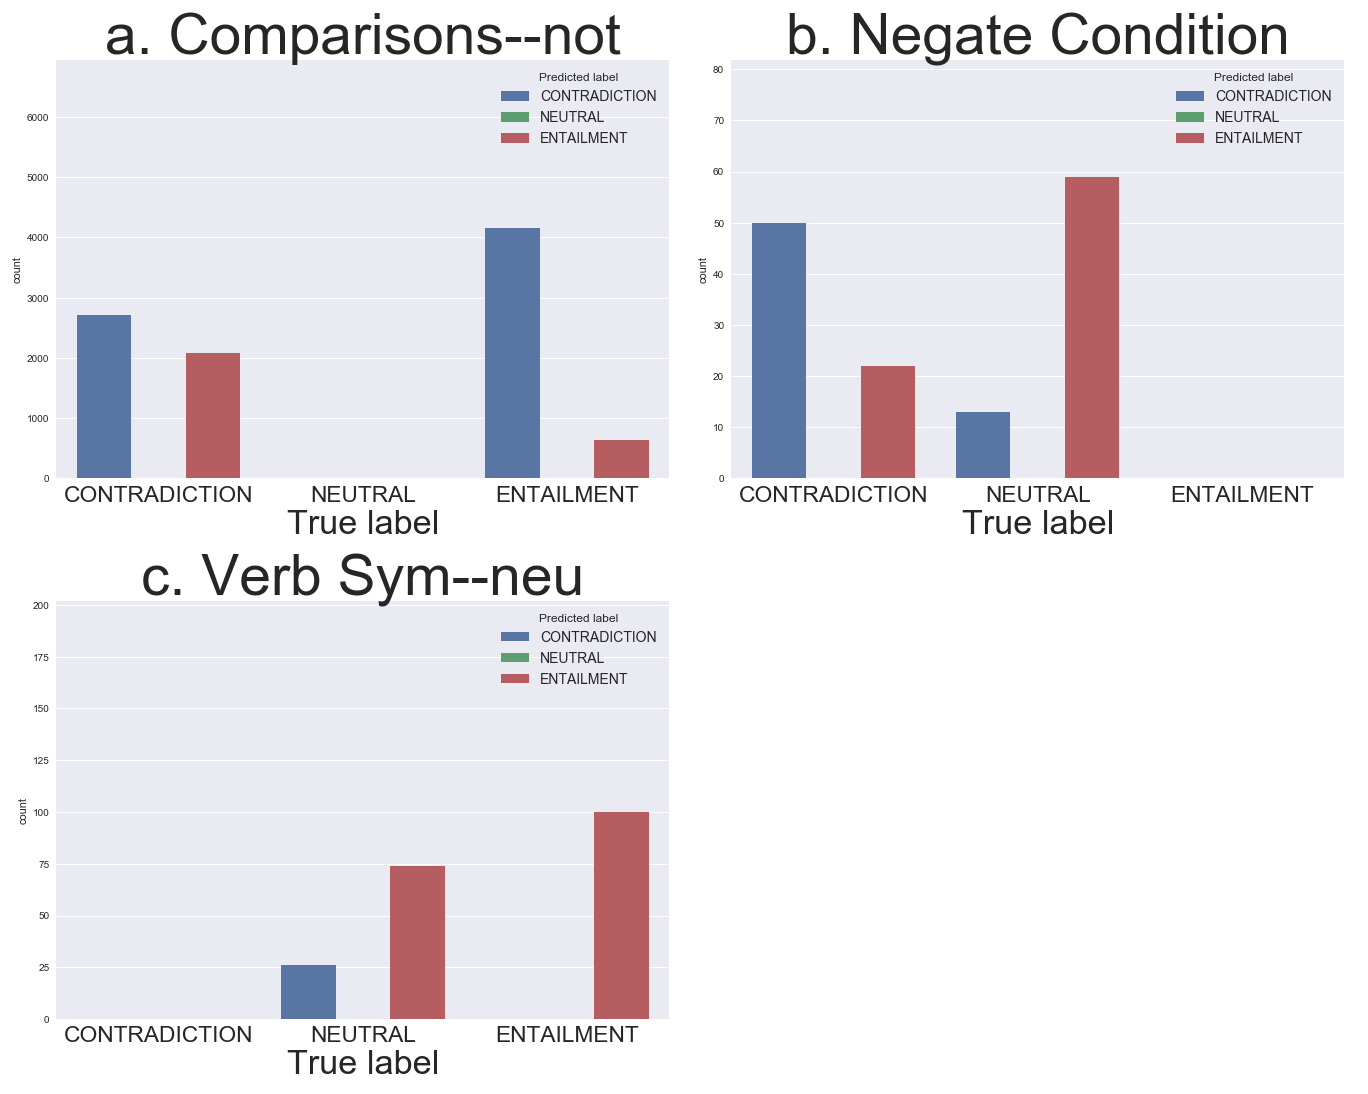
\includegraphics[width=0.45\textwidth]{NPShortHistsInferSentMLP.png}
\caption{Classifications by the MLP on the InferSent vectors with short noun phrases, tasks with `high asymmetry, low scores'.}
\label{fig:IShistMLP-NP}
\end{figure}


\begin{figure}[ht!]
\centering
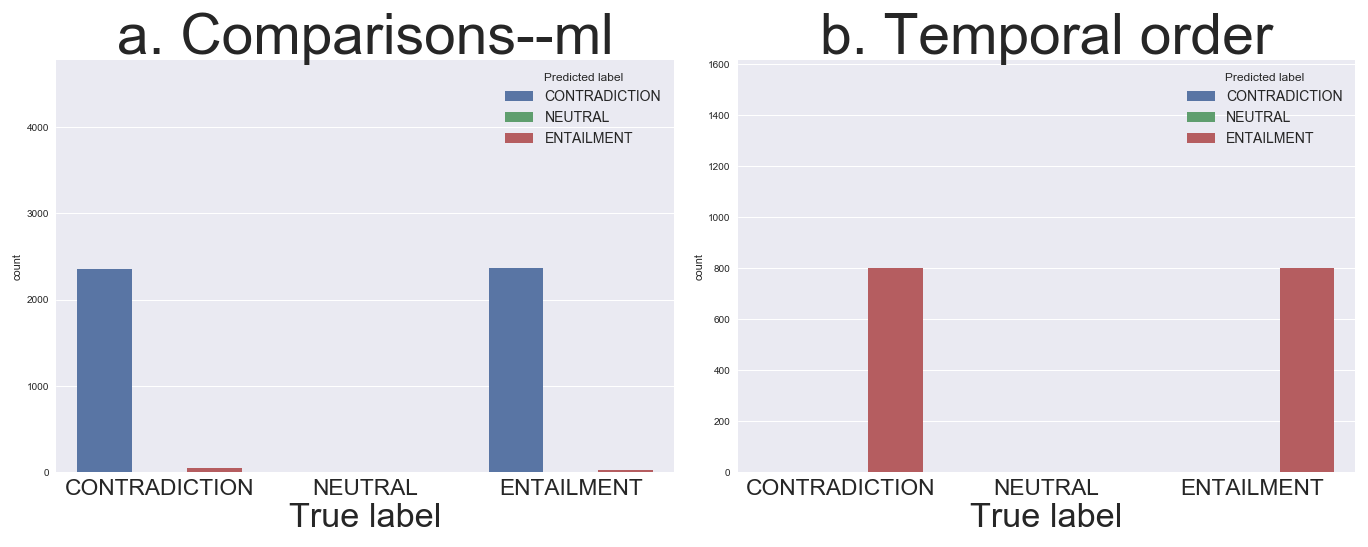
\includegraphics[width=0.45\textwidth]{NNShortHistsInferSentMLP.png}
\caption{Classifications by the MLP on the InferSent vectors with short noun phrases, tasks with `low asymmetry, low scores'.}
\label{fig:IShistMLP-NN}
\end{figure}

% Note: As the noun phrases get longer, InferSent always tends to classify them more as entailment, and BOW as neutral (the hatched red bar is always higher than the plain red bar in Infersent, and the hatched green bar is higher than unhatched green for BOW)


\section{Observations}

We analyse some of the patterns we observe and study the possible origins of this behavior based on the statstics of the SNLI dataset.

\subsubsection{All same words}
When the words in both sentences are the same, they are classified as entailing one another, except in the presence of certain words. 
We observe that in SNLI dataset, most contradictory sentence pairs have no overlap in words. It's much more likely for a sentence pair to be entailment or neutral if they have a lot of words overlap. For example, a contradictory sentence pair in SNLI is:\\
% @Demi: We should keep the format of how we present example sentences consistent. Also, is this example actually in SNLI?
{\tt A: Several people are trying to climb a ladder in a tree. \\ B: People are watching a ball game. \\ CONTRADICTION}

In order to qualitatively verify this observation, we rank all the sentence pairs by overlap rate: $\frac{\text{\# of overlap words}}{\text{total \# of words}}$(in non-increasing order). We then look at top X sentences with highest overlap (or \textit{relevance}), and we observe:

\begin{table}[htb]
  %%\centering
  \resizebox{\columnwidth}{!}{%
  \begin{tabular}{|l|l|l|l|}
  \hline
     Top &Entailment & Neutral & Contradiction \\
    \hline\hline
All & 183416 (33.4 \%) & 182764 (33.3 \%) & 183187 (33.3 \%) \\
\hline 
10000 & 3954 (39.5 \%) & 3567 (35.7 \%) & 2479 (24.8 \%)\\
\hline
 1000 & 508 (50.8 \%) & 407 (40.7 \%) & 85 (8.5 \%)\\
 \hline
  \end{tabular}}
 \caption{High Overlap of words in SNLI}
  \label{tab:highOverlap}
\end{table}

As shown in Table \ref{tab:highOverlap}, $91.5\%$ of the pairs with maximum overlap between the sentences have the true label of either entailment or neutral, and are very rarely labelled contradiction. 

\subsubsection{Difference of one word}

When the words in two sentences differ by just one word, the decision is largely based on if those words have opposing meanings irrespective of the order of the words. We see this from performance on more-less type comparisons (Figure \ref{fig:IShistMLP-NN}a). Here the words across the pairs differ only in the presence or absence of the word `more' or `less'. For example:\\
{\tt A: The woman is more cheerful than the man \\ B: The woman is less cheerful than the man\\ CONTRADICTION \\}{\tt A: The woman is more cheerful than the man \\ B: The man is less cheerful than the woman \\ ENTAILMENT} \\
Since the relation between the words `more' and `less' is largely contradictory, their use in pair of sentences leads the classifier to presume the sentences are contradictory, irrespective of the order of the words. 
%We further confirm this observation, to see that $60.0 \%$ sentence pairs that Infersent classified as contradiction contain antonyms.
% @Demi: What is the base rate of antonyms to compare this against? Or the rate for entailments?
% @Demi: Would be good to include where you get the antonym data set from - i.e. how do you know the sentences contain antonyms?


We now observe that this heuristic is fairly consistent with SNLI data. 
\begin{table}[htb]
  %%\centering
  \resizebox{0.9\columnwidth}{!}{%
  \begin{tabular}{|l|l|l|l|}
  \hline
    & P(Antonym $|$ X) & P( X $|$ Antonym) \\
    \hline\hline
    X = Contradiction & 12.2 \% & 61.2 \% \\
      X = Entailment &  3.5 \% &  18.0 \% \\
\hline 
  \end{tabular}}
 \caption{ Antonym word pair in the SNLI data set}
  \label{tab:antonyms}
\end{table}

We see in Table \ref{tab:antonyms} that the presence of antonyms strongly predicts a true label of contradiction in the SNLI data set. If we consider only the top 1000 in the high overlap set, the trend is more evident with $43.5 \%$ contradiction sentence pairs containing antonyms, and only $8.7 \%$ entailment sentence pairs containing antonyms. 

%We also find that the presence of antonyms that are most used in the SNLI data set are more likely to indicate contradiction for InferSent. For example, the antonyms  women/men, boy/girl and black/white appear more frequently in the SNLI sentence pairs than antonyms like old/young, sitting/standing, and sentences that differ by the first set of antonym pairs are more likely to be classified as contradiction by InferSent, than sentences that differ by the second set of antonym pairs.

\subsubsection{Negations}

We see that comparatives that differ in the presence  or absence of the negation `not', are largely classified as contradictions (Figure \ref{fig:IShistMLP-NP}a). To verify that our observation strongly correlates with SNLI train data, we look at sentence pairs that contain "negating ngrams": no, not, n't, don't, doesn't.
% @Demi aren't "don't, doesn't" redundant given "n't"?
\begin{table}[htb]
  %%\centering
  \resizebox{0.9\columnwidth}{!}{%
  \begin{tabular}{|l|l|l|l|}
  \hline
    & P(Negation $|$ X) & P( X $|$ Negation) \\
    \hline\hline
    X = Contradiction & 3.3 \% & 58.4 \% \\
      X = Entailment &  1.1 \% &  20.0 \% \\
\hline 
  \end{tabular}}
 \caption{Overall Data Negation statistics}
  \label{tab:negation}
\end{table}


We see in Table \ref{tab:negation} that the presence of negations strongly predicts a true label of contradiction in the SNLI data set. If we consider only the top x in the high overlap set, the trend is more evident. 
% @Demi: for both antonyms and negating, give either top 1000 or top 10,000 overlap statistics. top 10,000 here, top 1000 for antonyms.
We observe that $60.0 \%$ sentence pairs with negation are contradictions, and only $7.5 \%$ are entailment. \\

%Note that we also did same experiment on more broadly defined negation ngrams which includes Neither, None and etc, and we get similar results. We have $43.6\%$ negation pairs are contradiction, while $27.3\%$ negation pairs are entailment. $7 \%$ contradiction pairs have negation while only $4 \%$ entailment pairs have negation.



\begin{table*}[ht!]
  \centering
  \begin{tabular}{||l|l|p{85mm}|l|p{15mm}|p{15mm}||}
  \hline
     Data &Type & Sentences & True & IS-LR & BOW-LR \\
    \hline\hline
% \multirow{8}{*}{\parbox{1.2cm}{Scramble Test data}} & \multirow{2}{*}{VerbSym (cont)} & A: the boy overtakes the girl .\newline
% B: the boy overtakes the girl . & Entail & Entail (99.90\%) & Entail (77.82\%)\\ 
%  \cline{3-6}
%  && A: the boy overtakes the girl .\newline
% B: the girl overtakes the boy . & Contr & Contr (99.78\%) & Entail (77.82\%)\\ 
%  \cline{2-6}
 
%  & \multirow{2}{*}{Comp} & A: the girl is less cheerful than the boy . \newline
%  B: the girl is less cheerful than the boy .  & Entail & Entail (99.99\%) & Entail (69.13\%) \\ 
%  \cline{3-6}
%  && A: the girl is less cheerful than the boy . \newline
%  B: the boy is less cheerful than the girl . & Contr & Contr (94.75\%) & Entail (69.13\%) \\ 
%  \cline{2-6}
 
% %  &TempOrd & A: the woman in the black shirt stood up as the fat man frowned angrily. \newline
% %  B: the fat man frowned angrily as the woman in the black shirt stood up. & entail & entail (99..96\%) & neut (75.34\%) \\ 
% %  \cline{2-6}
% %  &Adj-Ref & A: The boy who is small , talks to the woman in the black shirt who is big.\newline
% %  B: The boy talks to the woman in the black shirt who is big. & entail & entail (99.55\%) & neut (71.78\%) \\ 
% %  \cline{2-6}

%  &\multirow{2}{*}{Subj-Verb} & A: the girl does shout loudly , however the fat man does not shout loudly . \newline
%  B: the fat man does not shout loudly .  & Entail & Entail (96.81\%) & Entail (73.39\%) \\
%  \cline{3-6}
%  & & A: the girl does not shout loudly , however the fat man does shout loudly . \newline
%  B: the fat man does not shout loudly .  & Contr & Contr (98.52\%) & Entail (73.39\%) \\
%  \cline{2-6}
 
%  &\multirow{2}{*}{NegCond} & A: the roads are dangerous when there are many clouds .\newline
%  B: the roads are dangerous when there are not many clouds . & Neut & Entail (58.63\%) & Entail (74.18\%)\\
%  \cline{3-6}
%  && A: the roads are dangerous when there are many clouds . \newline
%  B: the roads are not dangerous when there are many clouds . & Contr & Contr (90.58\%) & Entail (74.18\%)\\
%  \hline
%  \hline

  
\multirow{3}{*}{\parbox{1.2cm}{ SNLI data}} & \multirow{3}{*}{Test set } & A: A runner in a black and blue uniform competes in a race.\newline
 B: he is winning. & neut & neut (99.99\%) & contr (99.89\%) \\
 \cline{3-6}
&& A: A boy runs as others play on a homemade slip and slide. \newline
 B: A boy is running. & entail & entail (99.95\%) & contr (99.89\%) \\
 \cline{3-6}
 && A: A man sits at a table in a room. \newline
 B: A woman sits. & contr & contr (99.99\%) & entail (99.75\%) \\

 \hline
  \end{tabular}
  \caption{High Margin misclassifications by BOW}
  \label{tab:highMargin}
\end{table*}


\subsubsection{The effect of permuting}
So far we have focused on word level information in the statistics of SNLI in explaining much of InferSent's behavior. A systematic analysis of the effect of word order if challenging due to the combinatorial explosion in the number of possibilities. But we make a few observations.

In some cases, the order of words has no effect whatsoever on the classification made by InferSent, for example with temporal ordering type sentences (Figure \ref{fig:IShistMLP-NN}b).\\
{\tt  A: The woman stood up after the man stood up \\ B: The woman stood up after the man stood up \\ ENTAILMENT \\}{\tt A: The woman stood up after the man stood up \\ B: The man stood up after the woman stood up \\ CONTRADICTION}\\
This is perhaps because the SNLI dataset does not contain many time-ordered events, and has not learned the meanings of the words `before' and `after' and that they promote ordering, therefore defaulting to entailment due to the high overlap.\\
The presence of words/short N-grams that are known to contradict each other (`more X'/`less X', `is'/`is not', other antonyms), or just words that indicate order sensitivity (`more', `overtake'), seem to elicit some word order sensitivity for InferSent.  
From qualitative analysis, we observe that if common antonyms are swapped in order, then Infersent will likely classify this sentence pair as a contradiction. For example:
{\tt A: Boy sitting with a girl on the bench in the park \\ B: Girl sitting with a boy on the bench in the park}
%Moreover, we observe that when the order of common antonyms are swapped, then it's highly likely this is a contradiction in SNLI training dataset.
% @Demi: verify using quantitative data that above claims are correct
% TODO: check how confident InferSent is on temporal ordering classifications

We conjecture that simply a larger perturbation to the permutation of words (in the presence of these "order promoting" words) takes the classification closer to contradiction. This is trivially true for cases where zero perturbation results in an entailment inference, and a perturbation to order the order sometimes leads to a contradiction (same-type comparatives, verb-symmetries in Figures \ref{fig:IShistMLP-PP}c,e \ref{fig:IShistMLP-NP}c). But the key observation that supports this conjecture is in the case of comparatives of the `not' type \ref{fig:IShistMLP-NP}a. 
{\tt A: The woman is more cheerful than the man \\ B: The woman is not more cheerful than the man\\ CONTRADICTION \\}{\tt A: The woman is more cheerful than the man \\ B: The man is not more cheerful than the woman \\ ENTAILMENT} \\
Here, all pairs of sentences differ in the presence of `not', and as observed in the section on `negations' we see that all of these are more likely classified as contradictions than entailments. But in this dataset, pairs that more perturbed in the word order are in fact entailments. \\
We see the reverse trend in the classifications made by InferSent – sentences that are truly entailments, and are more perturbed in word order, are more likely to be classified as contradictions than true contradictions. Further, we also find that while all comparatives of the `more-less' type are classified as contradictions (Figure \ref{fig:IShistMLP-NN}a), the system is more confident about the ones that are truly entailment ($1867/2400$ pairs) being contradictions, i.e. the ones that have a larger perturbation to word order. 
%This could also perhaps explain why the `who-is' version of the adjective reference binding (Figure \ref{fig:IShistMLP-PP}b) shows a stronger effect than without (Figure \ref{fig:IShistMLP-PP}a), since one entails a larger perturbation to the order of the words because of the extra words `who is'.

\subsubsection{Other asymmetries}

InferSent perhaps encodes meanings of some ngrams. This is supported by asymmetry in subject-verb binding(Figure \ref{fig:IShistMLP-PP}d) \\
{\tt A: The woman stands up, however the man sits down \\ B: The woman stands up. \\ ENTAILMENT \\}{\tt A: The man stands up, however the woman sits down \\ B: The woman stands up. \\ CONTRADICTION}\\
Where the distinction requires the system to encode the binding of the words `woman sits' and `man stands'. It also shows asymmetry on adjective-reference binding(Figure \ref{fig:IShistMLP-PP}a)\\
{\tt A: The tall woman met the short man \\ B: The woman met the short man \\ ENTAILMENT \\}{\tt A: The tall woman met the short man \\ B: The short woman met the man \\ CONTRADICTION}\\
Where the binding for the word pairs `tall woman' and `short woman' are important. However, the performances on both of these is very low.

Also, perhaps the combining of a phrase with `not' is encoded. This could be argued from the asymmetry in negating a conditional (Figure \ref{fig:IShistMLP-NP}b).
\\
{\tt A: If there is a lot of snow, it is very cold \\ B: If there is a lot of snow, it is not very cold \\ CONTRADICTION \\}{\tt A: If there is a lot of snow, it is very cold \\ B: If there is not a lot of snow, it is very cold \\ NEUTRAL}\\
Where the binding of not with the different verb-phrases would allow for the observed asymmetry. However, the number of sentence pairs in this dataset is fairly low and is more difficult to draw conclusions from  %However, it could also be explained by sensitivity to where in the sentence the `not' occurs, with the first `is' or the second. 
%Performance on this tasks stays low. despite high asymmetry, due to misclassification of all the neutral pairs in the dataset as entailment.


\subsection{SNLI test set}

Our ScrambleTest set is not balanced, and was not part of the training. For a more controlled way to understand the differences between the performance of InferSent and Bow, we try to also look at the cases in the SNLI test set that are correctly classified by InferSent but incorrectly classified by BOW, with a high margin/confidence. See Table \ref{tab:highMargin} for examples. It seems from these that BOW learn contradiction only as `no overlap in words' whereas although InferSent is also strongly affected by the extent of overlap in words, it is able to have a more nuanced encoding (`man sits' vs `woman sits'). This also explains why BOW classifies almost all of the pairs in our data set as entailments, since most of the pairs in our dataset have a high overlap in the words used. Further, it also is able to encode meanings that straddle two or more words, for example that `runs' entails `is running'. This is consistent on what we observed about bi-grams above. However, it is difficult to make general claims. %A better understanding of what InferSent could achieve if also trained on some sentences from our ScrambleTests dataset that highlight the value of word-order and compositionality, is left to future work.

\section{Augmented training}
Now, we experiment with retraining the InferSent model on a combined dataset which includes both new ScrambleTest and original SNLI training data. \\
The new ScrambleTest data uses a similar generation process as our old ScrambleTest data. However, we only generate data of the `comparisons' type since the performance of InferSent on these is the most interpretable. The training dataste is generated as follows: we collect positive comparison phrases (p) such as "more adj." where "adj." is some adjective, and negative comparison phrases (n) such as "less adj.". The two sentences in a pair are of the form "(np1) is (p) than (np2)." and "(np2) is (n) than (np1).", where (np1) and (np2) are applicable noun phrases. The adjectives and noun phrases are randomly sampled from a large set of given possibilities. In total, we generated 40k such sentence pairs, which is roughly $7 \%$ of overall SNLI training data (550k sentence pairs).\\
Moreover, in order to minimize the effect of other factors such as vocabulary distribution. We intentionally modified our generation process, so that the vocabulary distribution of this newly generated ScrambleTest is similar to original SNLI training dataset. Only 7 words differ by more than %(@Demi : Is this right? Chnaged from "at leats 1%" because that was confusing) 
$1 \%$ in their occurrence in SNLI: not, a, than, the, is, less, more. \\


\section{Summary of findings}
The classifier based on InferSent definitely does not capture all of the compositionality in sentence structure. While it is difficult to pin down exactly what it is that the classifier does pick up on, certain behaviors draw attention to some potentially heuristic encodings of sentence compositionality. 

First, we see that the difference of one word between the two sentences, when the difference is an antonym or a negation, leads to InferSent tending to classify them as contradictions irrespective of word order. This is best highlighted in the more/less type and not type comparison dataset tests. This heuristic has ecological validity in the training set – as shown in Tables \ref{tab:antonyms} and \ref{tab:negation}, we see that the presence of negations and antonyms strongly correlate with a contradiction label. This illustrates a disproportionate dependence on lexical, rather than compositional meaning in InferSent. 

Second, in cases where even the words across the pairs are the same, we see that sometimes the order of the words is detected, and taken into account for the classification (as indicated in performance on the verb-symmetries and the same-type comparisons). This is sometimes detected and (correctly in this case) tagged a contradiction. However, for the not-type comparisons, the more jumbled pairs are in fact entailments. The classifier does the opposite, with true entailments (that is more jumbled ones) more often being classified as contradiction than the true contradictions. This hints at one way in which order information might be used, but is a heuristic that might often work. Finding ecological valididty for permutations in SNLI is challenging and we leave this to future work.

Finally, we see that there are some other cases in which InferSent performs above $50\%$, indicating that it is picking up some information about the relative positions of the words, although clearly not enough to perform competitively on these compositional tasks. Further work is needed to better isolate exactly what is learned, but is beyond the scope of this work.

This work demonstrates the inadequacy of most datasets available today in truly testing if compositional structure, i.e. structure beyond lexical structure, is being picked up by NLP models. InferSent achieves very high performance on the test set of the SNLI dataset, \textit{as well as several other tasks}, but fails on our dataset. Our ScrambleTest dataset is available online to test future models on. This work highlights the value of crafting diagnostic datasets, in the spirit of tasks designed in in cognitive psychology, in better understanding the behavior of these complex models. Our results on augmented training also show promise for systematic training sets... xyz.
% @Demi: todo, fill in trained network results

%Some of the sub-types, particularly comparisons, adjective-referent binding, and subject-verb binding have enough sentence pairs to be able to consider including some of them during training to augment the classifier. We leave this to future work.

\section{Future Directions}

This is one step towards building better diagnostic test sets to score NLI models like InferSent. Other interesting things to try would be to see how other models, particularly generative models like SkipThought, differ on these metrics. Further, we could use more sophisticated methods like LIME (Local Interpretable Model-Agnostic Explanations, \cite{ribeiro2016should}) to generate interpretable explanations for its classifications and understand the performance of these models on diagnostic datasets. 



%\begin{itemize}
%\item How much info do the sentence representations actually have?
%\begin{itemize}
%\item BOW: How much is lost due to averaging, and to what extent is it possible to back out the words? Include `product of all word reps' and other (?) operations that are symmetric to word position to improve info transfer about words in the sentence as a \textbf{fairer BOW baseline comparison}.
%\item InferSent: Could a decoder recreate the sentence from the last hidden state of an RNN? 
%\end{itemize}
%\item Are the ScrambleTests examples just too different from SNLI to make a fair comparison?
%\begin{itemize}
%\item Train on part of the ScrambleTest data, ensuring no overfitting and retest.
%\item Ensure that distributional characteristics (base rates of words for eg, and other statistics) are comparable to SNLI.
%\end{itemize}
%\item What are the differences between the results from LogReg and MLP?
%\item Test other sentence representations 
%\item Find more precisely:
%\begin{itemize}
%\item Description of incremental compositional information needed and how different types of scrambled data sets provide a paving.
%\item What exactly InferSent classifies based on (LIME?). But perhaps that's getting too invested in InferSent in particular.
%\end{itemize} 
%\end{itemize}

\bibliographystyle{apa-good}
\bibliography{library}

\newpage
\section*{Other Figures}

\begin{figure}[ht!]
\centering
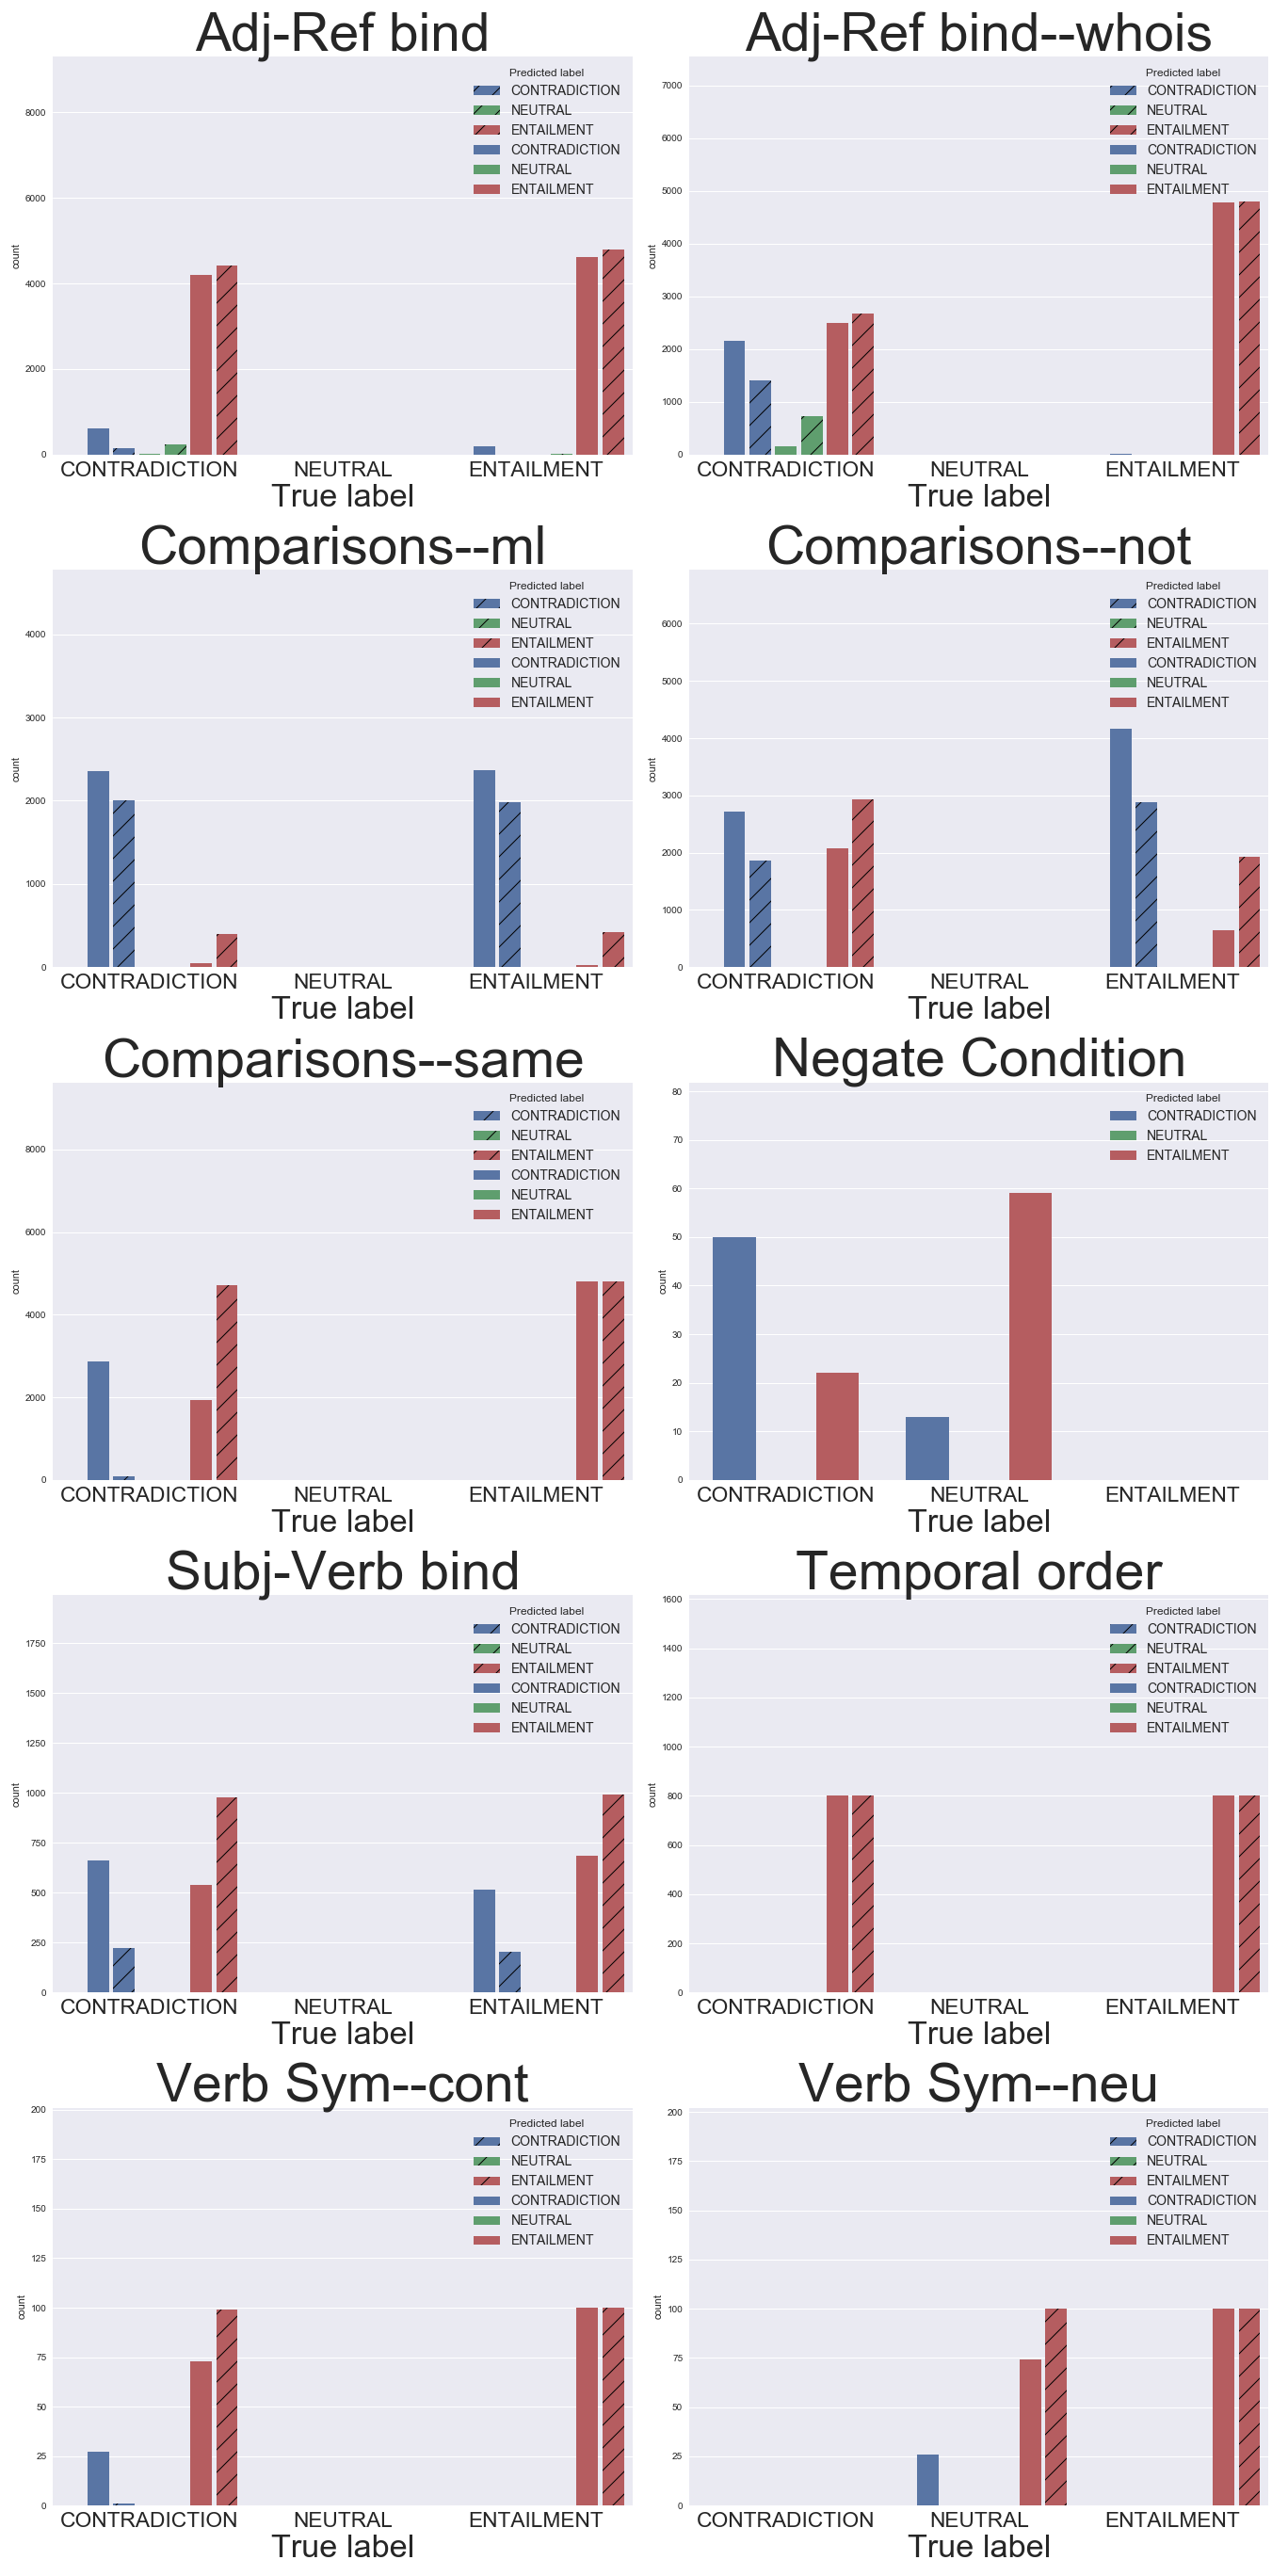
\includegraphics[width=0.45\textwidth]{AllHistsInferSentMLP.png}
\caption{ScrambleTest Data: The classifications made by the MLP on the InferSent vectors. Long noun phrases are hatched.}
\label{fig:IShistMLP}
\end{figure}


\begin{figure}[ht!]
\centering
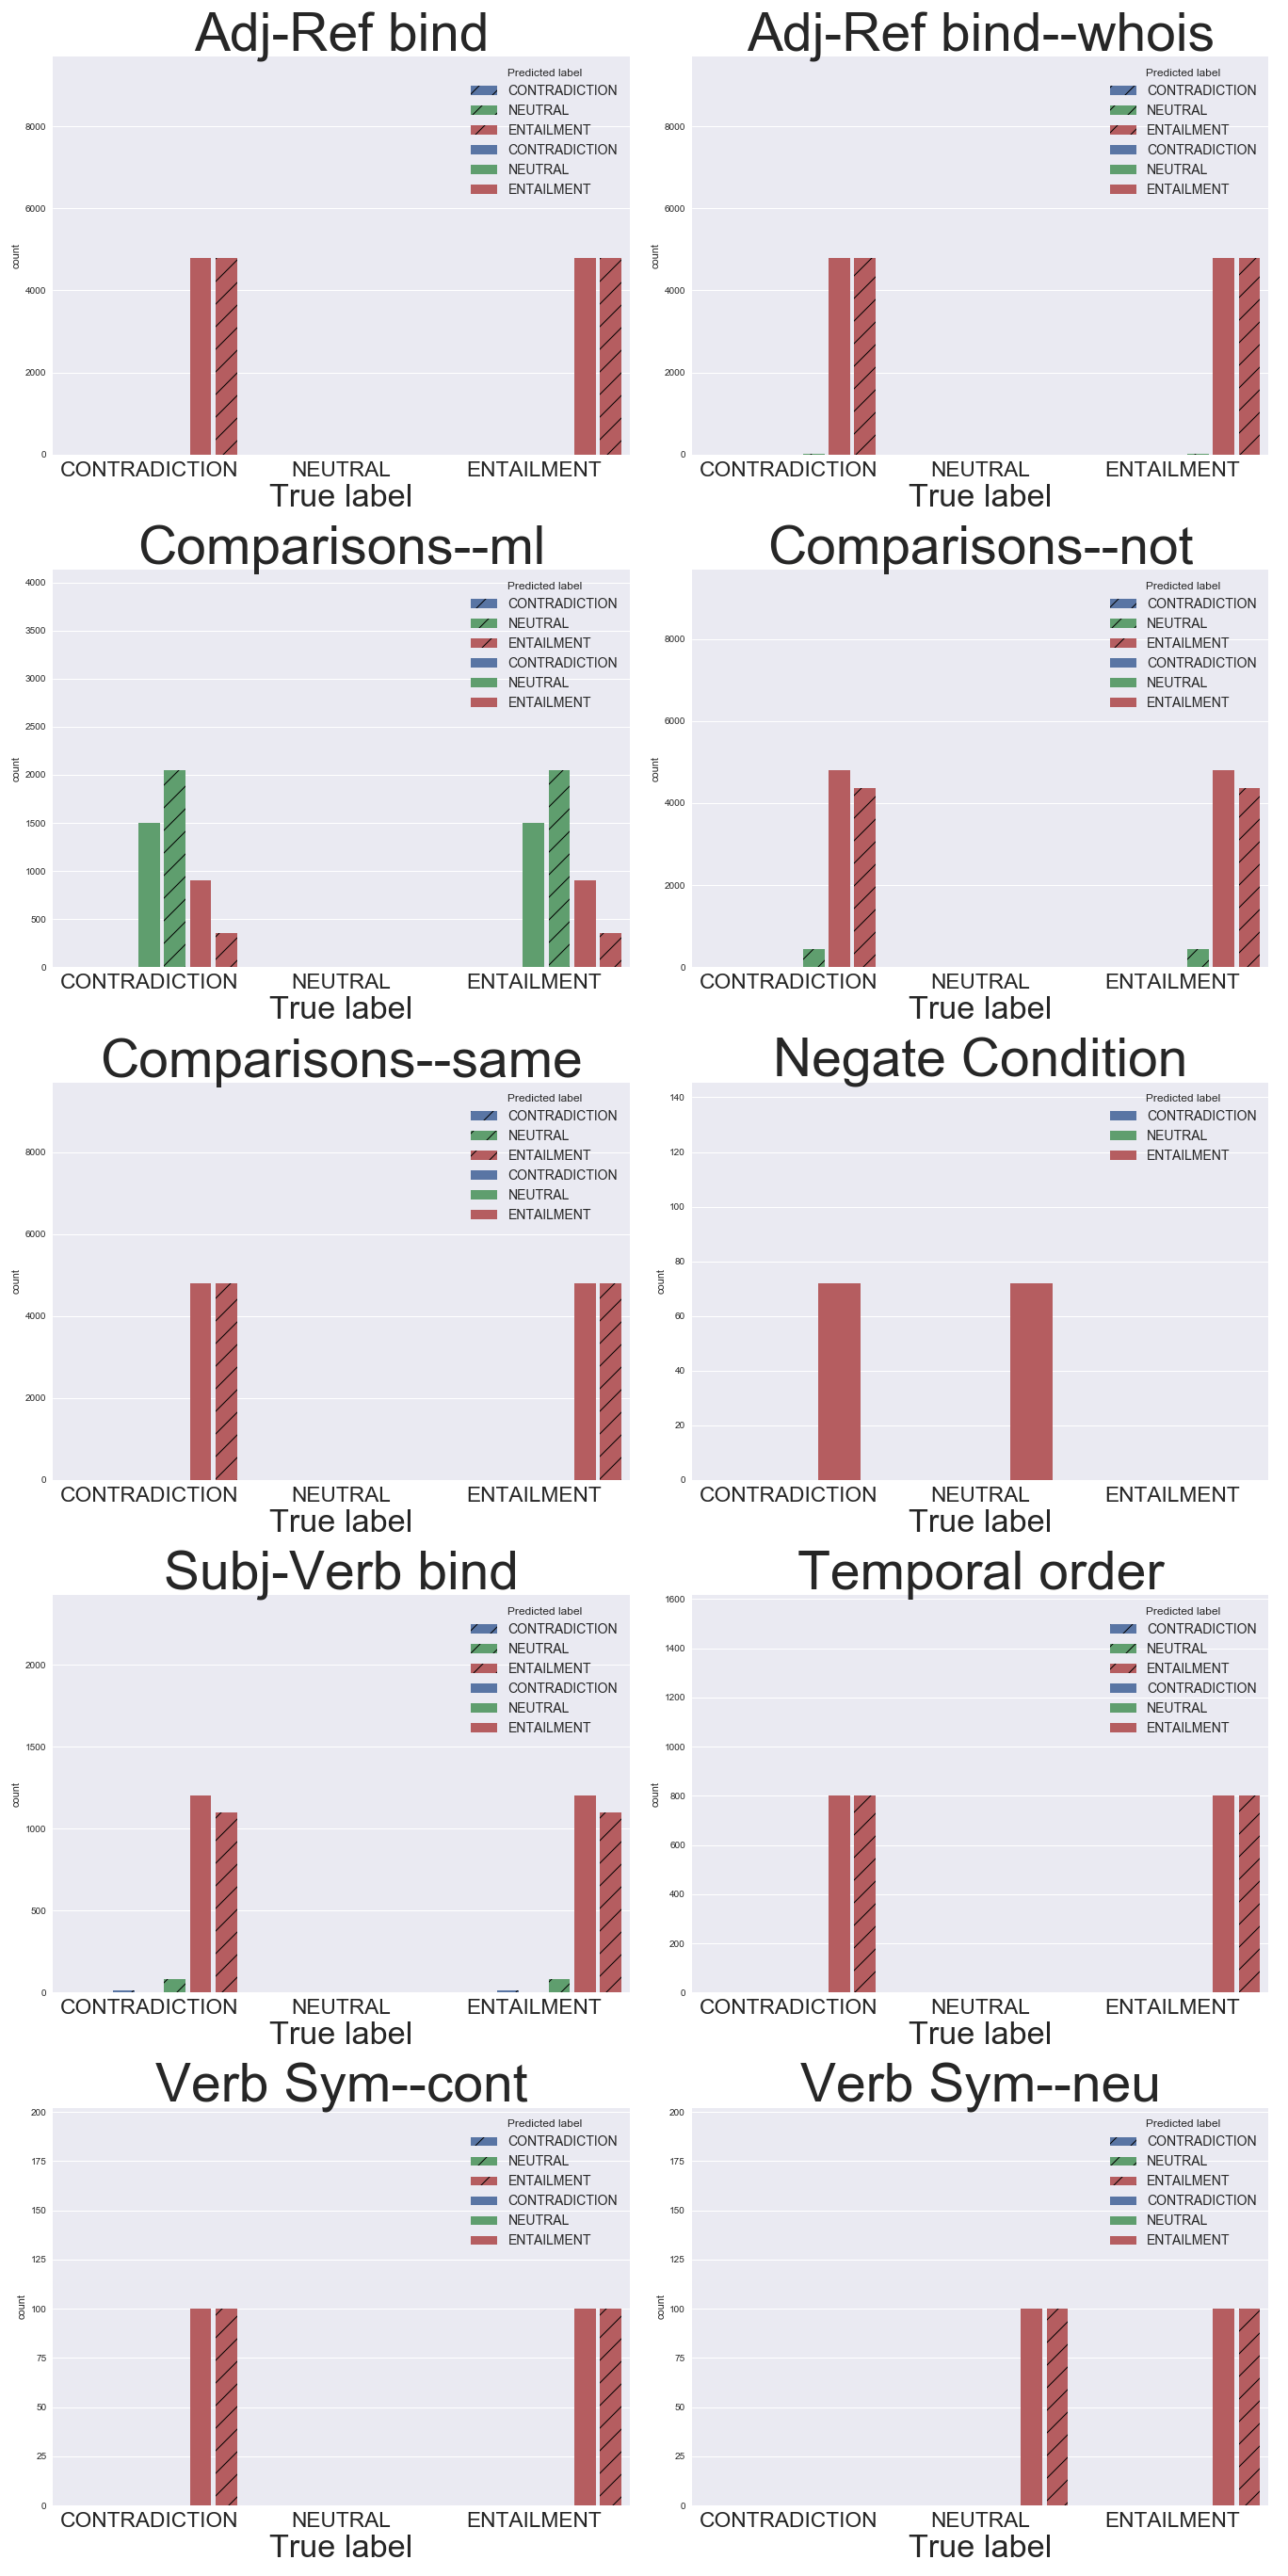
\includegraphics[width=0.45\textwidth]{AllHistsBOWMLP.png}
\caption{ScrambleTest Data: The classifications made by the MLP on the BOW vectors. Long noun phrases are hatched. Note that judgments are symmetric for both kinds of true labels, by design.}
\label{fig:BOWhistMLP}
\end{figure}



\begin{figure}[ht!]
\centering
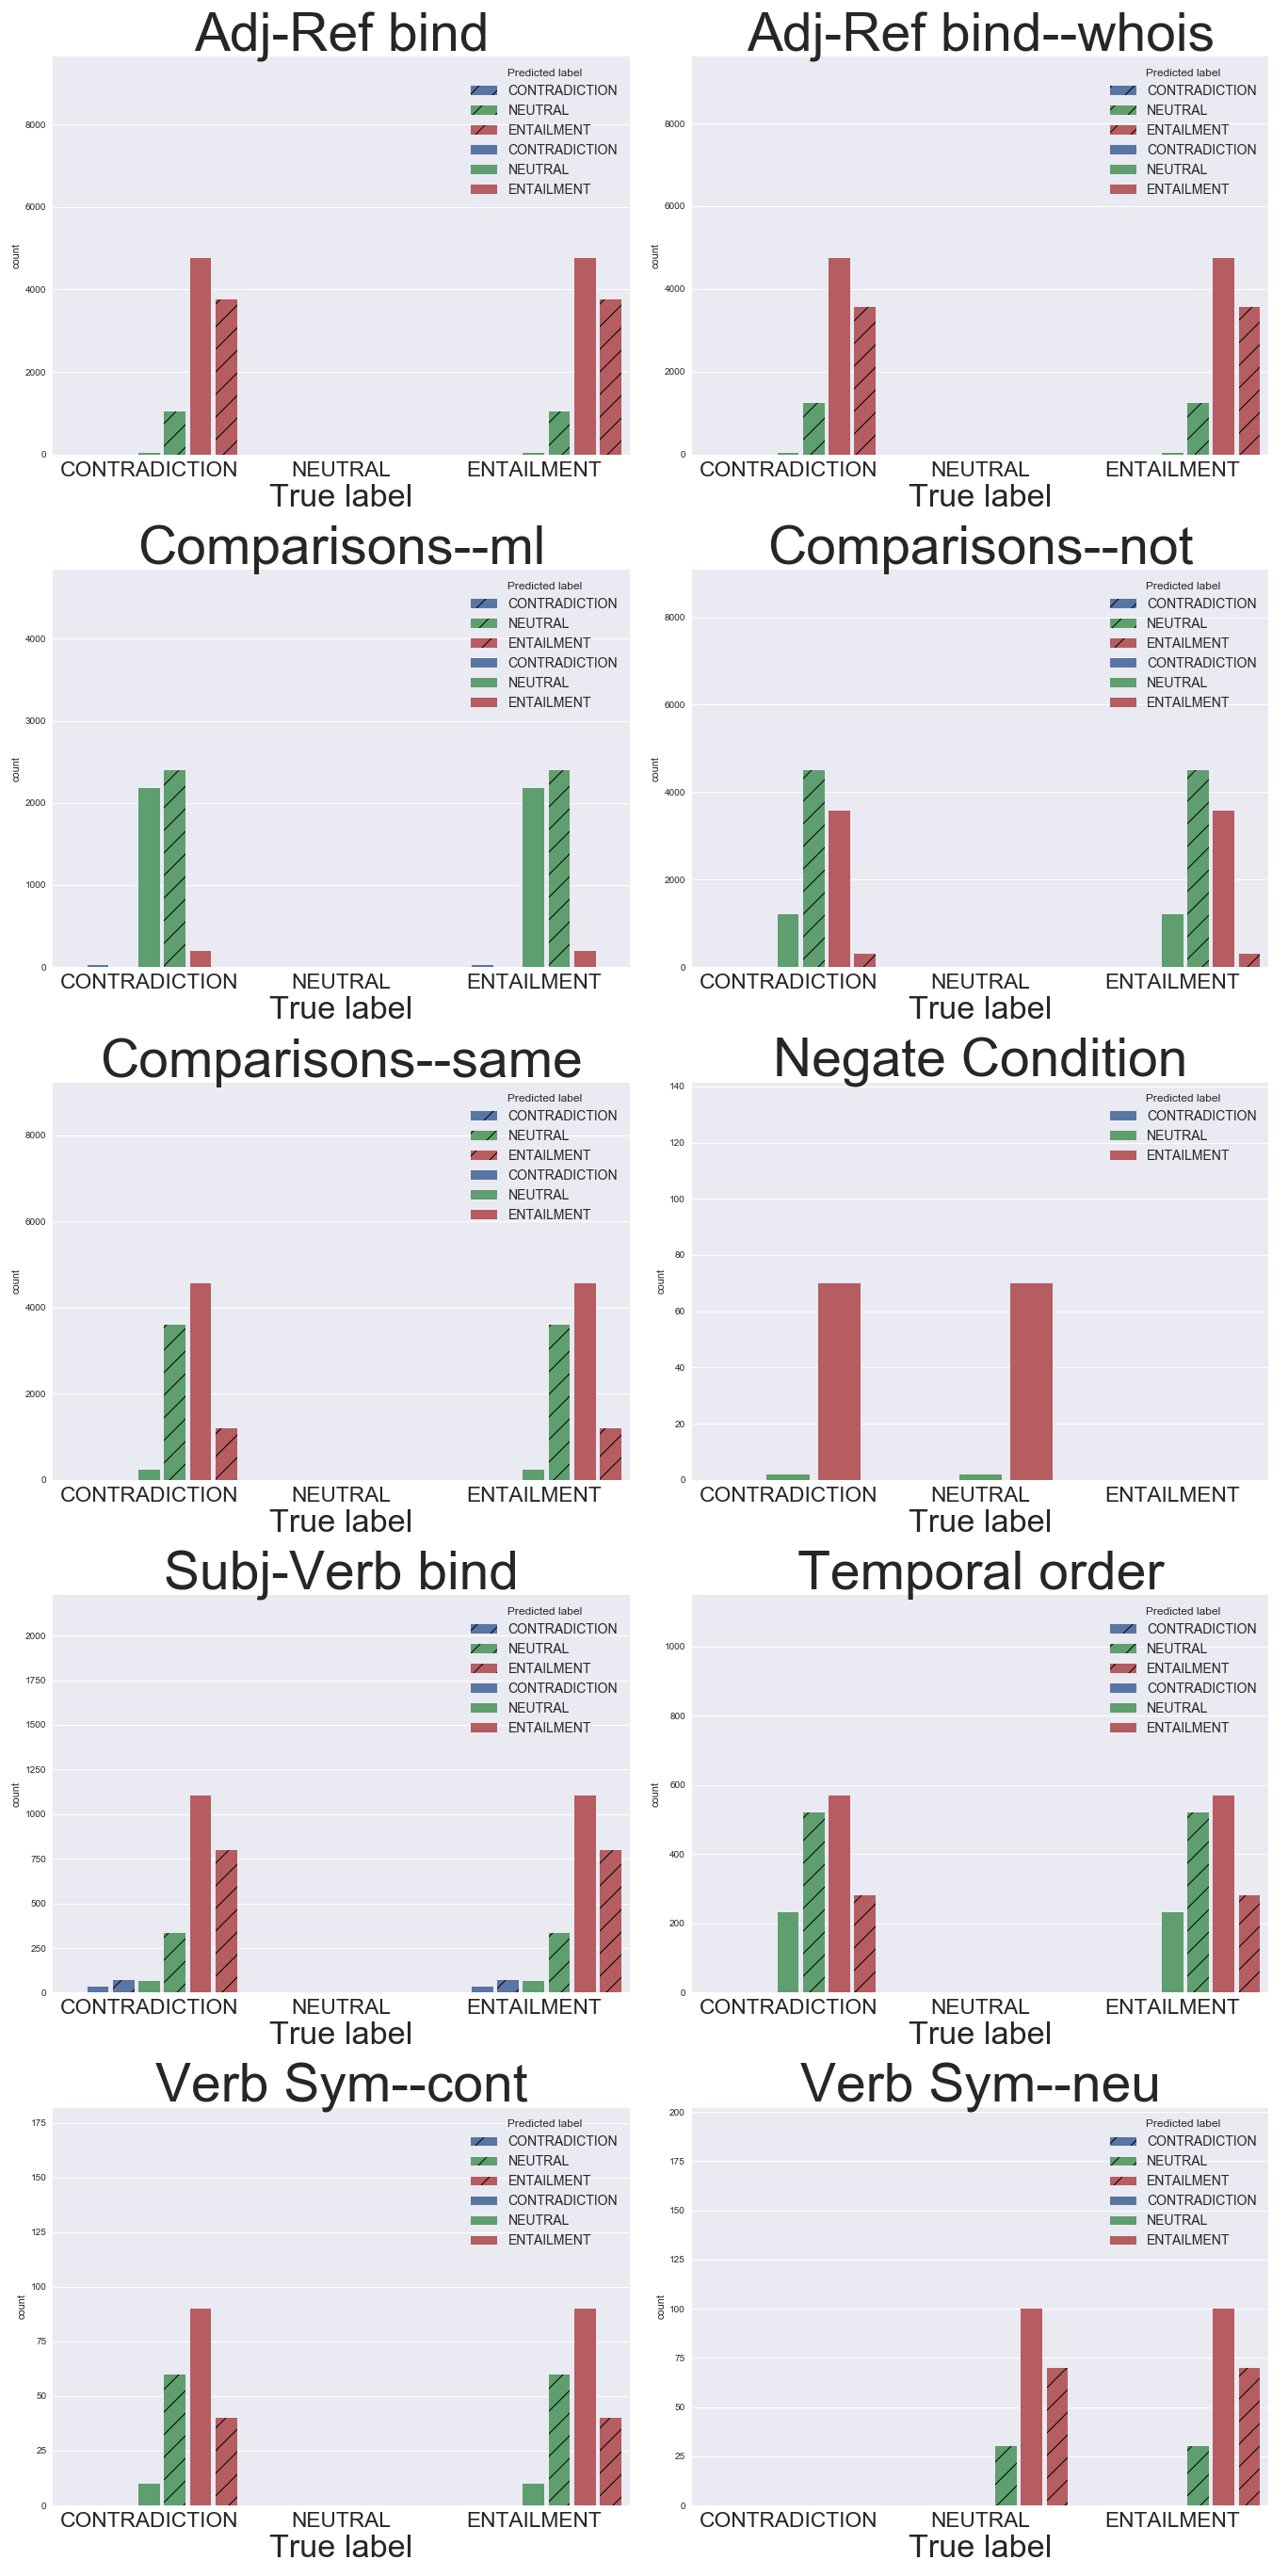
\includegraphics[width=0.45\textwidth]{AllHistsBOWLogReg.png}
\caption{ScrambleTest Data: The classifications made by the logistic regression on the BOW vectors. Long noun phrases are hatched.}
\label{fig:BOWhistLR}
\end{figure}



\begin{figure}[ht!]
\centering
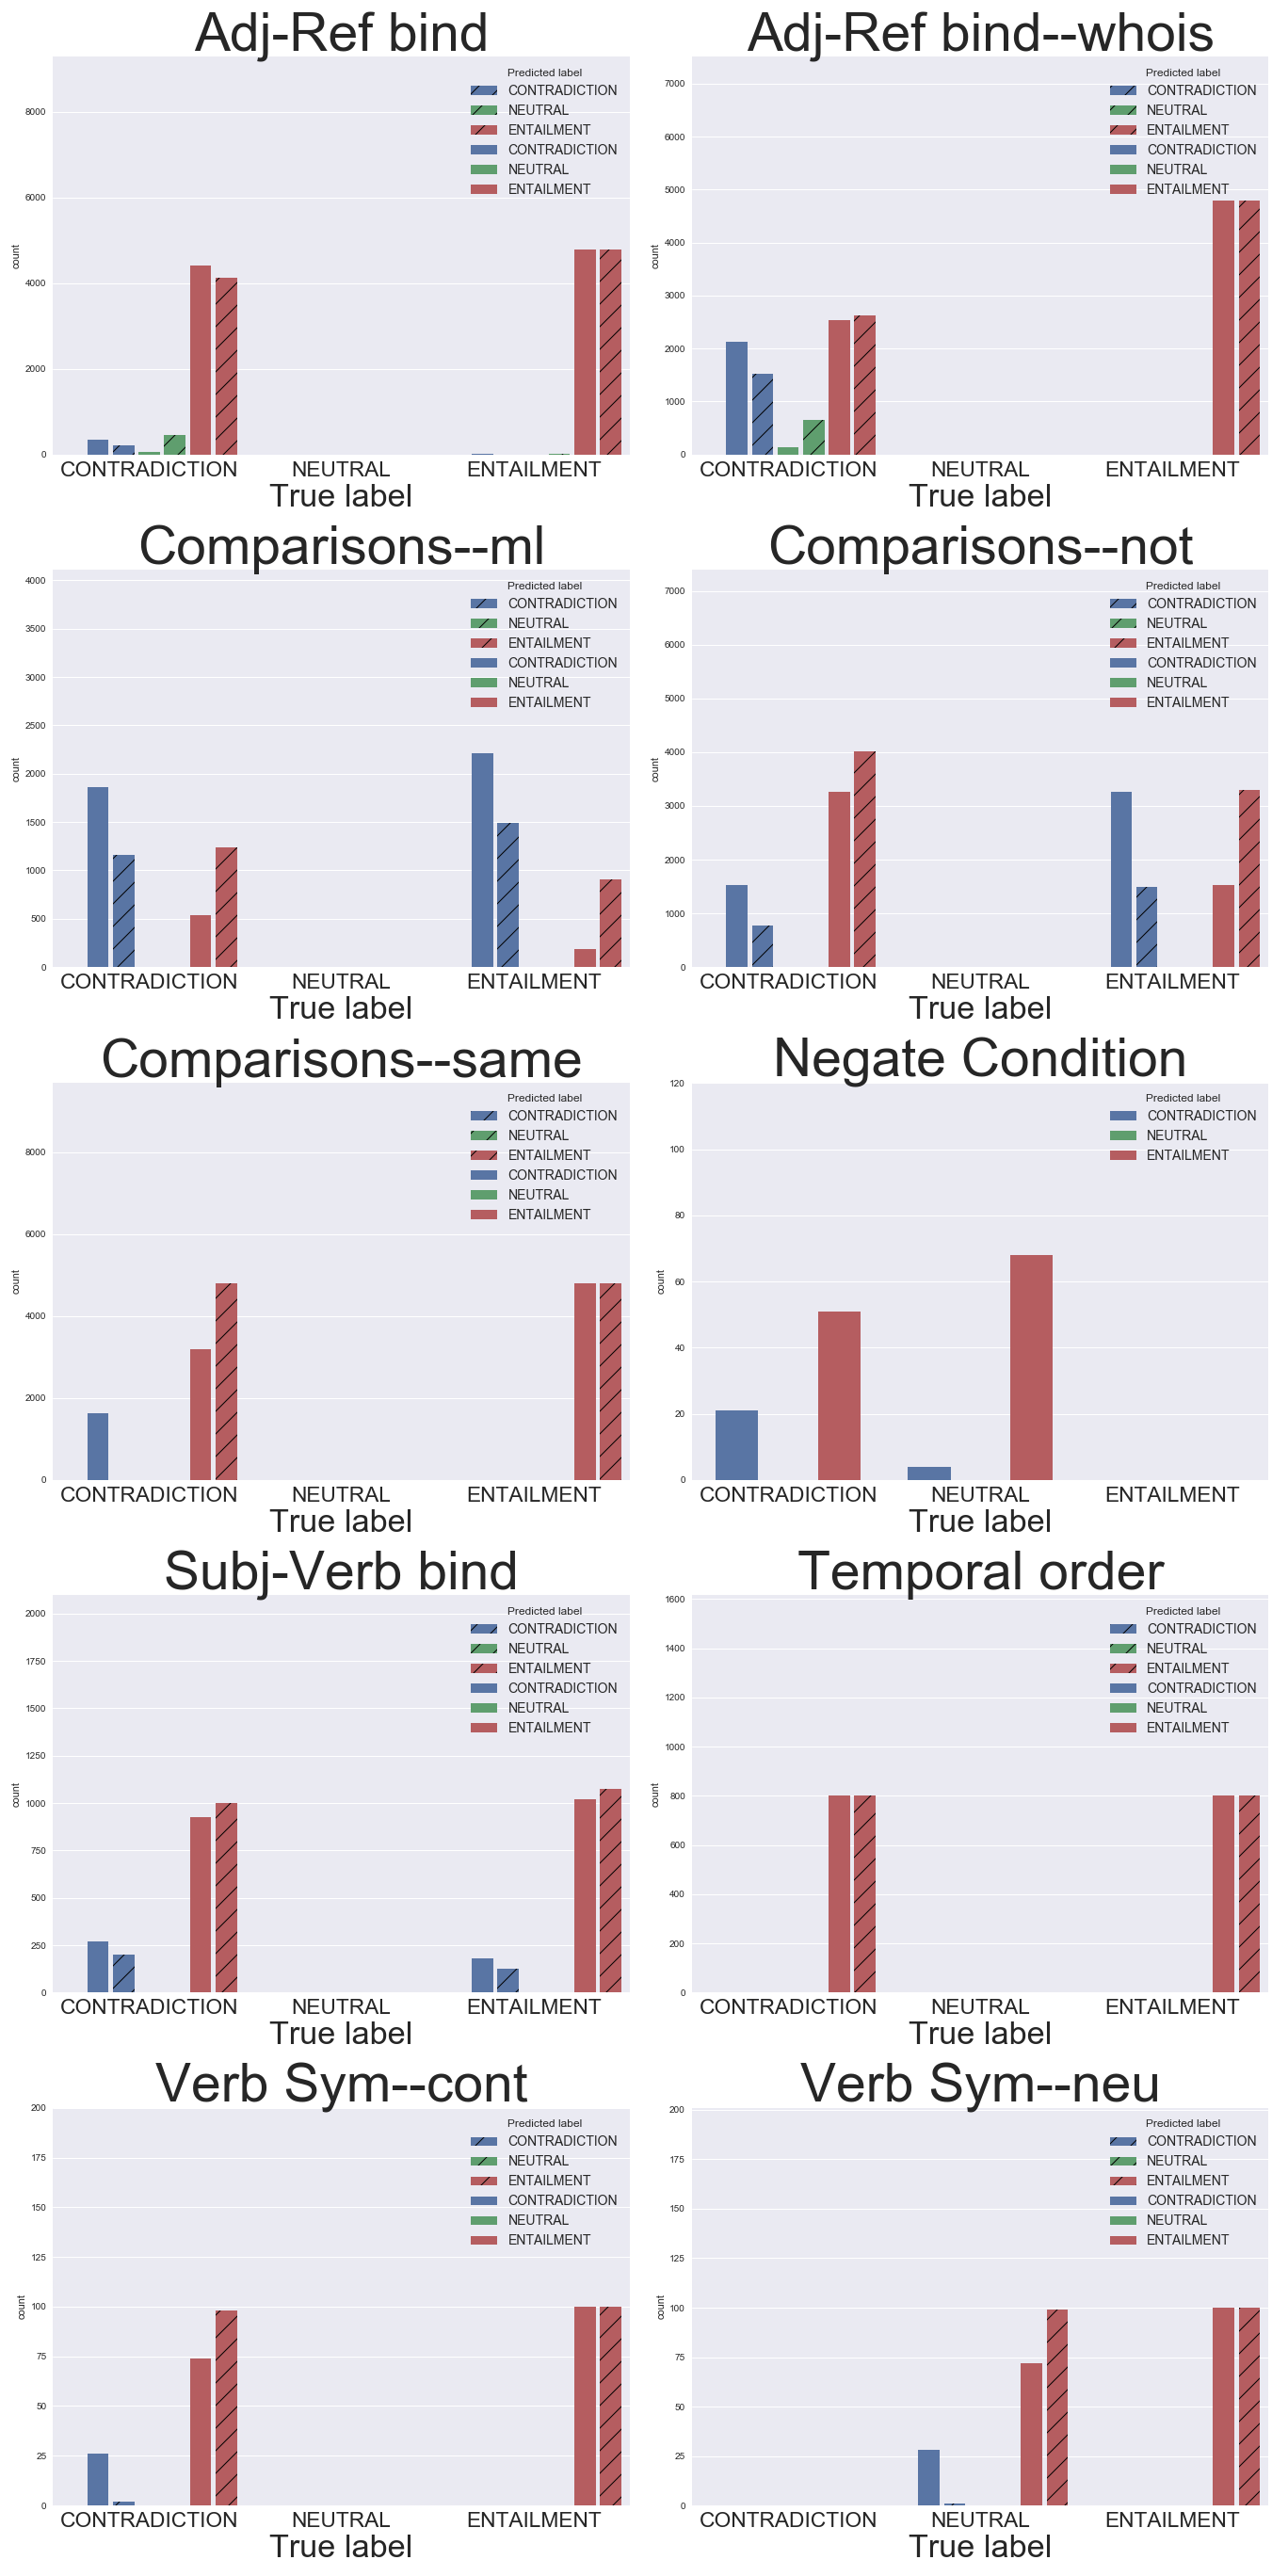
\includegraphics[width=0.45\textwidth]{AllHistsInferSentLogReg.png}
\caption{ScrambleTest Data: The classifications made by the logistic regression on the InferSent vectors. Long noun phrases are hatched.}
\label{fig:IShistLR}
\end{figure}

\end{document}

% \subsection{Adjective-Reference Binding}
% We see that in the vanilla case, almost everything is classified as entailment. When the explicit `who is' prompt is provided, performance improves. The perturbation is higher, i.e. the difference between the pairs of sentences is larger when the whole phrase `who is X' is moved to a different subject as opposed to if just the word 'X' is moved. The fact that classification as `neutral' also goes up in this case supports the hypotheses that the improved performance might just be from `who is' causing a larger perturbation (not necessarily directed towards the the boundary with `contradiction' cases) and therefore resulting in a re-assignment.

% \subsection{Comparisons}

% We see that in both the `more/less' and the `not' kind of questions, where the pairs differ in the words used, by swapping out `more' for `less', and either containing the word `not' or not, a very large number of them are classified as contradictions. This indicates that most of the decision is based on the fact that the pairs contain words that contradict each other, though the specific order of the words should (half the time) give rise to an entailment. This explains the low (less than 50\%) performance on these types. An interesting observation is that BOW does not classify these as contradictions, indicating that just the difference in the existence of the words `more' or `less' / the presence or absence of the word `not' across the sentence pairs does not drive this. Perhaps InferSent learns that the existence of `more' + \textit{some adjective} in one sentence and `less' + \textit{some adjective} in the other, drives a contradiction. That is, there in some understanding beyond just single words.

% The classifier does much better on the pairs of sentences in which the words are just scrambled (where no word information differs). Here, it has a tendency to classify almost everything as an entailment, but for short noun phrases, it does get quite a few of the contradictions correct (giving the highest performance across the board).

% \subsection{Negate Condition}

% Infersent performs very poorly on this task, mostly because it considers several of the true neutral as entailment. It is worth noting that it preferentially classifies the true contradiction as a contradiction. 

% We notice that in general, InferSent does not classify most of the sentences in our dataset as neutral.
% A possible explanation for this could be that the SNLI dataset was built on MTurk with the instructions for neutral being explicitly to be neutral to a description given. As a result, perhaps several neutral pairs have close to no overlap in the words used -- it is a lot easier to say neutral statement by just saying something generic, since a random description is more likely to be neutral than entail or contradict. For example, ``A couple play in the tide with their young son.'' is neutral with ``The family is on vacation.'' It's possible therefore that the system learns that a neutral ensues when there is low overlap in words used, which is never the case in our examples, explaining why the classifier never predicts a neutral \todo{But why does BOW predict neutral more?}. 

% \subsection{Subject-Verb Binding}
% Although the performance on this task is not very high, the classifier (for short noun phrases) does predict the correct response with greater than $50\%$ accuracy. For longer noun phrases, it mostly predicts entailment.

% \subsection{Temporal Order}
% The classifier always predicts entailment. This may be because, due to the way the SNLI data corpus has been collected (captioning photos), there are not very many temporally ordered events for the classifier to learn the meanings of words like `before' and `after'

% \subsection{Verb Symmetry}
% The pairs that are not classified entailments, are very similarly classified across the two types (`contradiction' and `neutral' types). Some of the contradictions in the `contradiction' type are correctly classified while none of the neutrals are, leading to the performance gap. 

% \begin{figure}[ht!]
% \centering
% 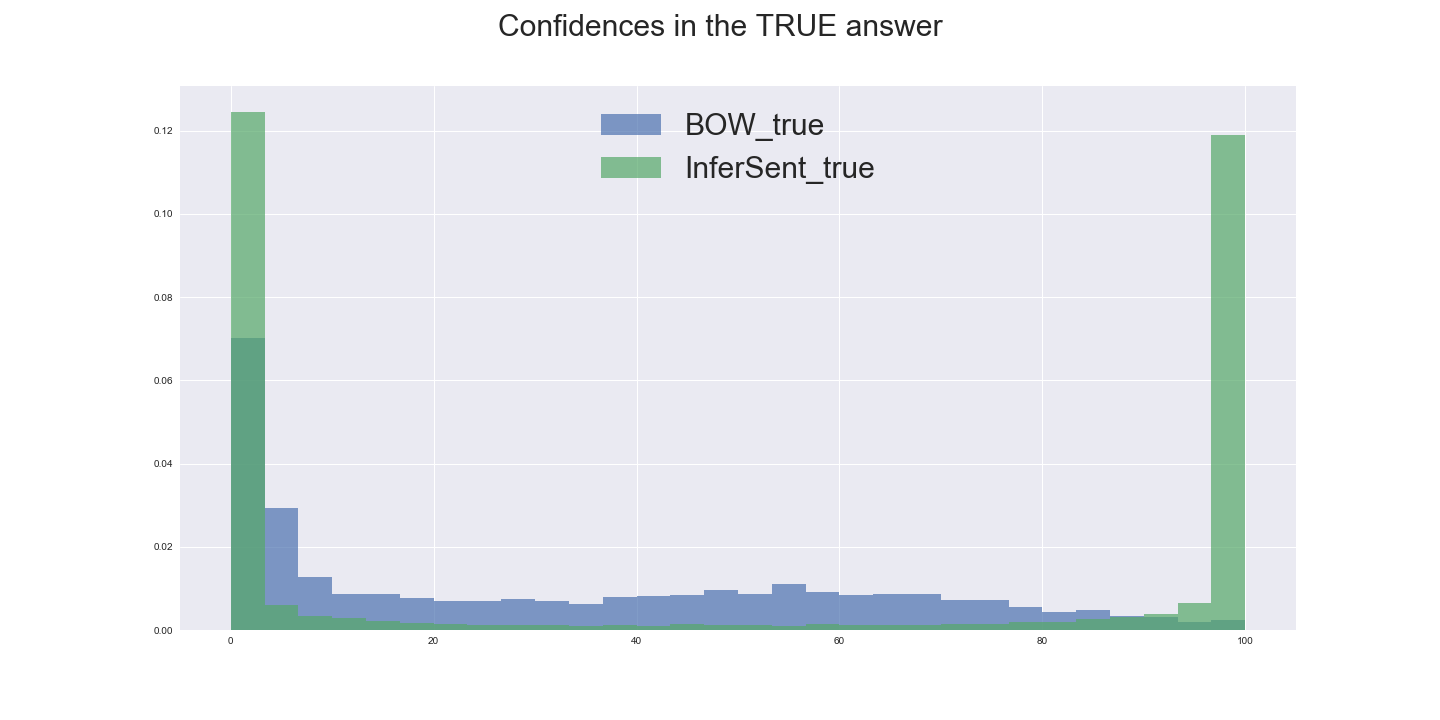
\includegraphics[width=0.40\textwidth]{conf_in_true.png}
% \caption{ScrambleTest Data: Confidences of the classifiers in the true answer.}
% \label{fig:truConf}
% \end{figure}


% \section{Confidence in answers}
% The confidences that each of these classifiers has in the true answer is not as easily distinguished by the true label for the SNLI test set (Figures \ref{fig:SNLIBOWconf_split} and \ref{fig:SNLIISconf_split}), as we can when tested on our dataset (particularly for BOW), indicating that these differences in confidence we see on our test set (Figures \ref{fig:BOWconf_split} and \ref{fig:ISconf_split}) are a feature of our scramble-test set and not the learned classifier. \todo{Why is BOW consistently more confident about entailments in the scrambleset?}
